%% ★ 국방발표 판 --- 본문은 sections_def/ 의 압축판을 읽는다. 저널 투고판
%%   (USV_swarm_defense_EAAI_KR_real.tex, sections_real/)은 손대지 않는다.
%%   변경 없는 파일(주제어·선언문·참고문헌·tables/)은 sections_real 을 공유한다.
%% ★ 도판은 figs_snak/real/ 을 real 판과 공유한다 --- 파일명을 바꾸면 real 판이 깨지므로
%%   재번호하지 않고, 발표판에서 안 쓰는 번호는 건너뛴다(본문 그림 번호는 LaTeX 가 등장
%%   순서대로 다시 매긴다). 도판은 기동 계층·체계 전체의 주장에만 둔다.
% !TEX program = xelatex
%==============================================================================
%  자폭 USV 군집 방어 — EAAI 투고용 한글 원고 (full paper)
%
%  이 파일은 SNAK 요약본(USV_swarm_defense_paper_CNN.tex)과 **별개**다.
%  요약본은 방법 소개가 전부이고 결과 절이 없다. 이 원고는 EAAI(Engineering
%  Applications of Artificial Intelligence)의 관례에 맞춰 검증을 무게중심으로 둔다:
%  관련연구·문제정의·실험설계·결과·고찰·한계가 전부 신규다.
%
%  조판: 2단. 큰 표(전 지표 10행×6열)와 가로로 긴 결과 도판은 table*/figure* 로
%       양단 걸침 처리한다. 표제·초록은 twocolumn[...] 으로 양단에 낸다.

%
%  컴파일: xelatex 3회 (상호참조 해결)
%       xelatex USV_swarm_defense_EAAI_KR.tex
%
%  ★ 표는 손으로 쓰지 않는다. tools/make_paper_tables.py 가 results/eval_merged/
%    의 CSV 에서 tables/*.tex 를 굽고 여기서 \input 한다. 평가를 다시 돌리면
%    표가 자동으로 맞는다. 표 안의 숫자를 직접 고치면 원자료와 어긋난다.
%==============================================================================
\documentclass[10pt,twocolumn]{article}

%------------------------------------------------------------------ 용지·판면
\usepackage[papersize={210mm,297mm}, left=20mm, right=20mm,
            top=22mm, bottom=22mm, columnsep=7mm]{geometry}

%------------------------------------------------------------------ 한글 글꼴
\usepackage{kotex}
\usepackage{fontspec}
% TeX Gyre Termes 는 TeX Live 에 항상 포함된다(시스템 폰트 의존 없음).
% 한글은 함초롬바탕 — fc-list 로 설치 확인함. 없는 PC 에서는 {Batang} 으로 바꾼다.
\setmainfont{TeX Gyre Termes}[Ligatures=TeX]
% ★ 함초롬 계열에는 이탤릭 자형이 없다. AutoFakeSlant 를 주지 않으면 본문의
%   \emph{강조} 한글이 조용히 정체로 떨어진다(로그: TU/HCRBatang(0)/m/it undefined).
%   본문에서 \emph 로 논지를 구분하므로 반드시 필요하다.
\setmainhangulfont{HCR Batang}[AutoFakeBold=2.0, AutoFakeSlant=0.2]
\setsanshangulfont{HCR Dotum}[AutoFakeBold=2.0, AutoFakeSlant=0.2]

%------------------------------------------------------------------ 패키지
\usepackage{amsmath, amssymb}
\usepackage{graphicx}
\usepackage{booktabs}          % \toprule 등 — tables/*.tex 가 요구한다
\usepackage{array}
\usepackage{multirow}          % 지표 표의 관점 열 병합
\usepackage{rotating}          % 부록의 전면 가로 도판(sidewaysfigure*)
\usepackage{caption}
\usepackage{subcaption}
\usepackage{float}
% ── float 배치 완화 ──────────────────────────────────────────────────────
%   twocolumn 에서 figure* 는 정의된 쪽에 못 들어가고 다음 쪽 상단으로만 간다. 양단
%   그림이 연달아 나오면 큐가 막혀 절 끝(또는 문서 끝)까지 밀린다 — 실제로 §4 본문
%   (5–11쪽)의 그림 11장이 21–27쪽에 떨어졌다. 아래 세 가지로 푼다.
\usepackage{dblfloatfix}        % figure* 를 쪽 하단에도 허용 + 순서 꼬임 방지
\renewcommand{\topfraction}{0.92}
\renewcommand{\bottomfraction}{0.70}
\renewcommand{\dbltopfraction}{0.92}
\renewcommand{\textfraction}{0.05}
\renewcommand{\floatpagefraction}{0.75}
\renewcommand{\dblfloatpagefraction}{0.75}
\setcounter{topnumber}{3}
\setcounter{dbltopnumber}{3}
\setcounter{totalnumber}{5}
\setcounter{topnumber}{3}
\setcounter{dbltopnumber}{3}
\setcounter{totalnumber}{5}
\usepackage[section]{placeins}  % 절이 바뀌면 남은 float 를 먼저 흘려보낸다
\raggedbottom                   % 2단에서 단 바닥을 억지로 맞추느라 제목 사이 여백이 늘어나는 것을 막는다
\usepackage{xcolor}
\usepackage{setspace}
\usepackage[numbers,sort&compress]{natbib}
\usepackage[hidelinks]{hyperref}
%% ★ 발표판: 표 밑 주석(각 표의 minipage 블록)을 싣지 않는다. tables/*.tex 는 자동
%%   생성물이라 손대지 않고 여기서 환경 자체를 비운다. 되살리려면 아래 두 줄을 지운다.
%%   (이 원고의 minipage 사용처가 표 주석뿐임을 확인하고 적용하였다.)
\usepackage{environ}
\RenewEnviron{minipage}[1]{}
\usepackage{enumitem}

% 한글 원고이므로 abstract 환경의 표제를 한글로. (article 클래스 기본은 "Abstract".)
\renewcommand{\abstractname}{초\;\;록}

\graphicspath{{figs_snak/real/}}   % ★ real 판: 이 폴더의 fig1~fig19 만 쓴다. 옛 파일이 남으면
                                   %   일부러 빌드가 실패하게 두었다(폴백 경로 없음).

\captionsetup{font=small, labelfont=bf, skip=6pt}
\captionsetup[table]{position=above}
\setstretch{1.06}
\setlength{\parskip}{2pt}

% 본문에서 반복되는 표기
\newcommand{\capr}{\mathrm{CR}}                     % 포획률
\newcommand{\dz}{d_z}
% \ensuremath 로 감싸 본문·수식 어디서나 쓸 수 있게 한다. 감싸지 않으면 본문에서
% "\mathrm allowed only in math mode" 로 컴파일이 깨진다.
% 자동 생성 표(tables/*.tex)는 투고판과 공유하므로 손대지 않는다. 발표판은 캡션만
% 짧은 명사구로 덮어써서 읽는다 --- 표를 다시 구워도 이 캡션은 유지된다.
\newcommand{\shortcaptext}{}
\newcommand{\inputshortcap}[2]{%
  \begingroup
  \renewcommand{\shortcaptext}{#1}%
  \let\origcaption\caption
  \renewcommand{\caption}[1]{\origcaption{\shortcaptext}}%
  \input{#2}%
  \endgroup}

\newcommand{\unit}[1]{\ensuremath{\,\mathrm{#1}}}

%==============================================================================

% 단 폭(≈232pt)보다 긴 식은 TeX 가 번호를 다음 줄로 내린다. 그런 식만 글자 크기를 한 단계
% (\small, 0.9배) 또는 두 단계(\footnotesize, 0.8배) 줄여 번호가 같은 줄에 남게 한다.
% 어느 식이 밀리는지는 scratchpad/eqcheck.py 로 전수 측정했다(2026-09-16).
\newenvironment{equationsmall}{\small\begin{equation}}{\end{equation}}
\newenvironment{equationfn}{\footnotesize\begin{equation}}{\end{equation}}

\begin{document}

\title{\bfseries 군집 자폭 수상 드론 방어를 위한\\
LLM 기반 지휘체계와 U-Net 점수맵 기반\\
다중 에이전트 협력 강화학습}

\author{윤영준\thanks{충남대학교} \and 방현태\footnotemark[1] \and
        전유라\thanks{한국과학기술원} \and 김덕환\footnotemark[2] \and
        윤원근\footnotemark[1]}
\date{}
% 2단 조판에서 표제·초록은 양단 걸침으로 낸다. 좁은 단에 초록이 들어가면
% 문단이 잘게 쪼개져 읽히지 않는다.
\twocolumn[\begin{@twocolumnfalse}
\maketitle
%============================================================ 초록 (압축판)
%  국방발표 판 전용. 모델명·세부 수치를 줄이고 주장 한 개당 수치 한 개로 둔다.
\begin{abstract}
\noindent
저비용 자폭 무인수상정(USV) 군집은 전자전이 유선 조종 표적에 닿지 않고 요격탄은 표적보다
비싸 포화되는, 재래식 대응의 사각지대에 있다. 본 연구는 적보다 느린 소수의 방어정이 모선의
접근 회랑을 그물벽으로 선제 차단하는 두 계층 방어 체계를 제안한다. 전략 계층에서는 대규모
언어모델(LLM) 지휘관이 방어정별 담당 무리를 정하고, 기동 계층에서는 U-Net 이 전장 격자
지도 위에 낸 점수맵에서 각 방어정이 픽셀을 지목해 그물벽 위치를 정한다. 두 계층은 같은
주기로 결정하지만 응답 지연이 크게 달라 느린 전략 계층만 비동기로 분리한다. 픽셀 지목은
행동공간을 격자에 가두어 안전·임무 제약을 마스킹으로 직접 부과하고 적선 수에 불변이며,
학습은 가치망 없는 그룹 상대 정책 최적화를 다중 에이전트로 확장한다. 8개 조건 $\times$ 3개
포메이션 $\times$ 30개 시드, 720 에피소드를 시드 대응표본으로 수집해 두 계층의 기여를
$2\times2$ 로 분리 측정하였다. 기동 계층은 언어모델 없이 단독으로 포획률을
$0.844 \to 0.886$ 으로 높였고, 제안 체계 전체는 같은 방어 수준에서 포획당 그물 소모를
45\,\%, 총 선회량을 47\,\% 줄였으며, 두 계층의 기여는 상승이 아닌 가산적이었다.
지휘관의 이득은 능력 임계를 넘는 모델에서만 나타났고, 그 성능을 설명한 것은 배정
커버리지가 아니라 재계획 간 계획 안정성이었다. 주기적으로 재계획하는 구조에서는 국소
최적성보다 시간에 걸친 일관성이 중요하다.
\end{abstract}

%============================================================ 주제어 (자작 조판본 전용)
%  elsarticle 판은 sections/00d_keywords.tex 의 keyword 환경을 쓴다.
%  이 파일은 옛 2단 자작 조판본(USV_swarm_defense_EAAI_KR.tex)이 계속 컴파일되도록 남긴다.

\vspace{4pt}
\noindent\textbf{주제어}\;: 무인수상정, 군집 방어, 다중 에이전트 강화학습, 임무배정, 대규모 언어모델, 의미론적 분할, 그룹 상대 정책 최적화

\vspace{10pt}

%% 하이라이트는 넣지 않는다 --- Elsevier 전용 요소이고, 이 자작 2단 조판본은
%% 국내 논문 형식의 기준 원고다. EAAI 투고본(USV_swarm_defense_EAAI.tex)에는
%% elsarticle 의 highlights 환경으로 들어가고, 별도 제출 파일은
%% tools/make_highlights.py 가 논문초안/highlights.{txt,tex} 로 뽑는다.
\vspace{8pt}
\end{@twocolumnfalse}]
%============================================================ 1. 서론 (압축판)
\section{서론}
\label{sec:intro}

\begin{figure*}[tp]
\centering
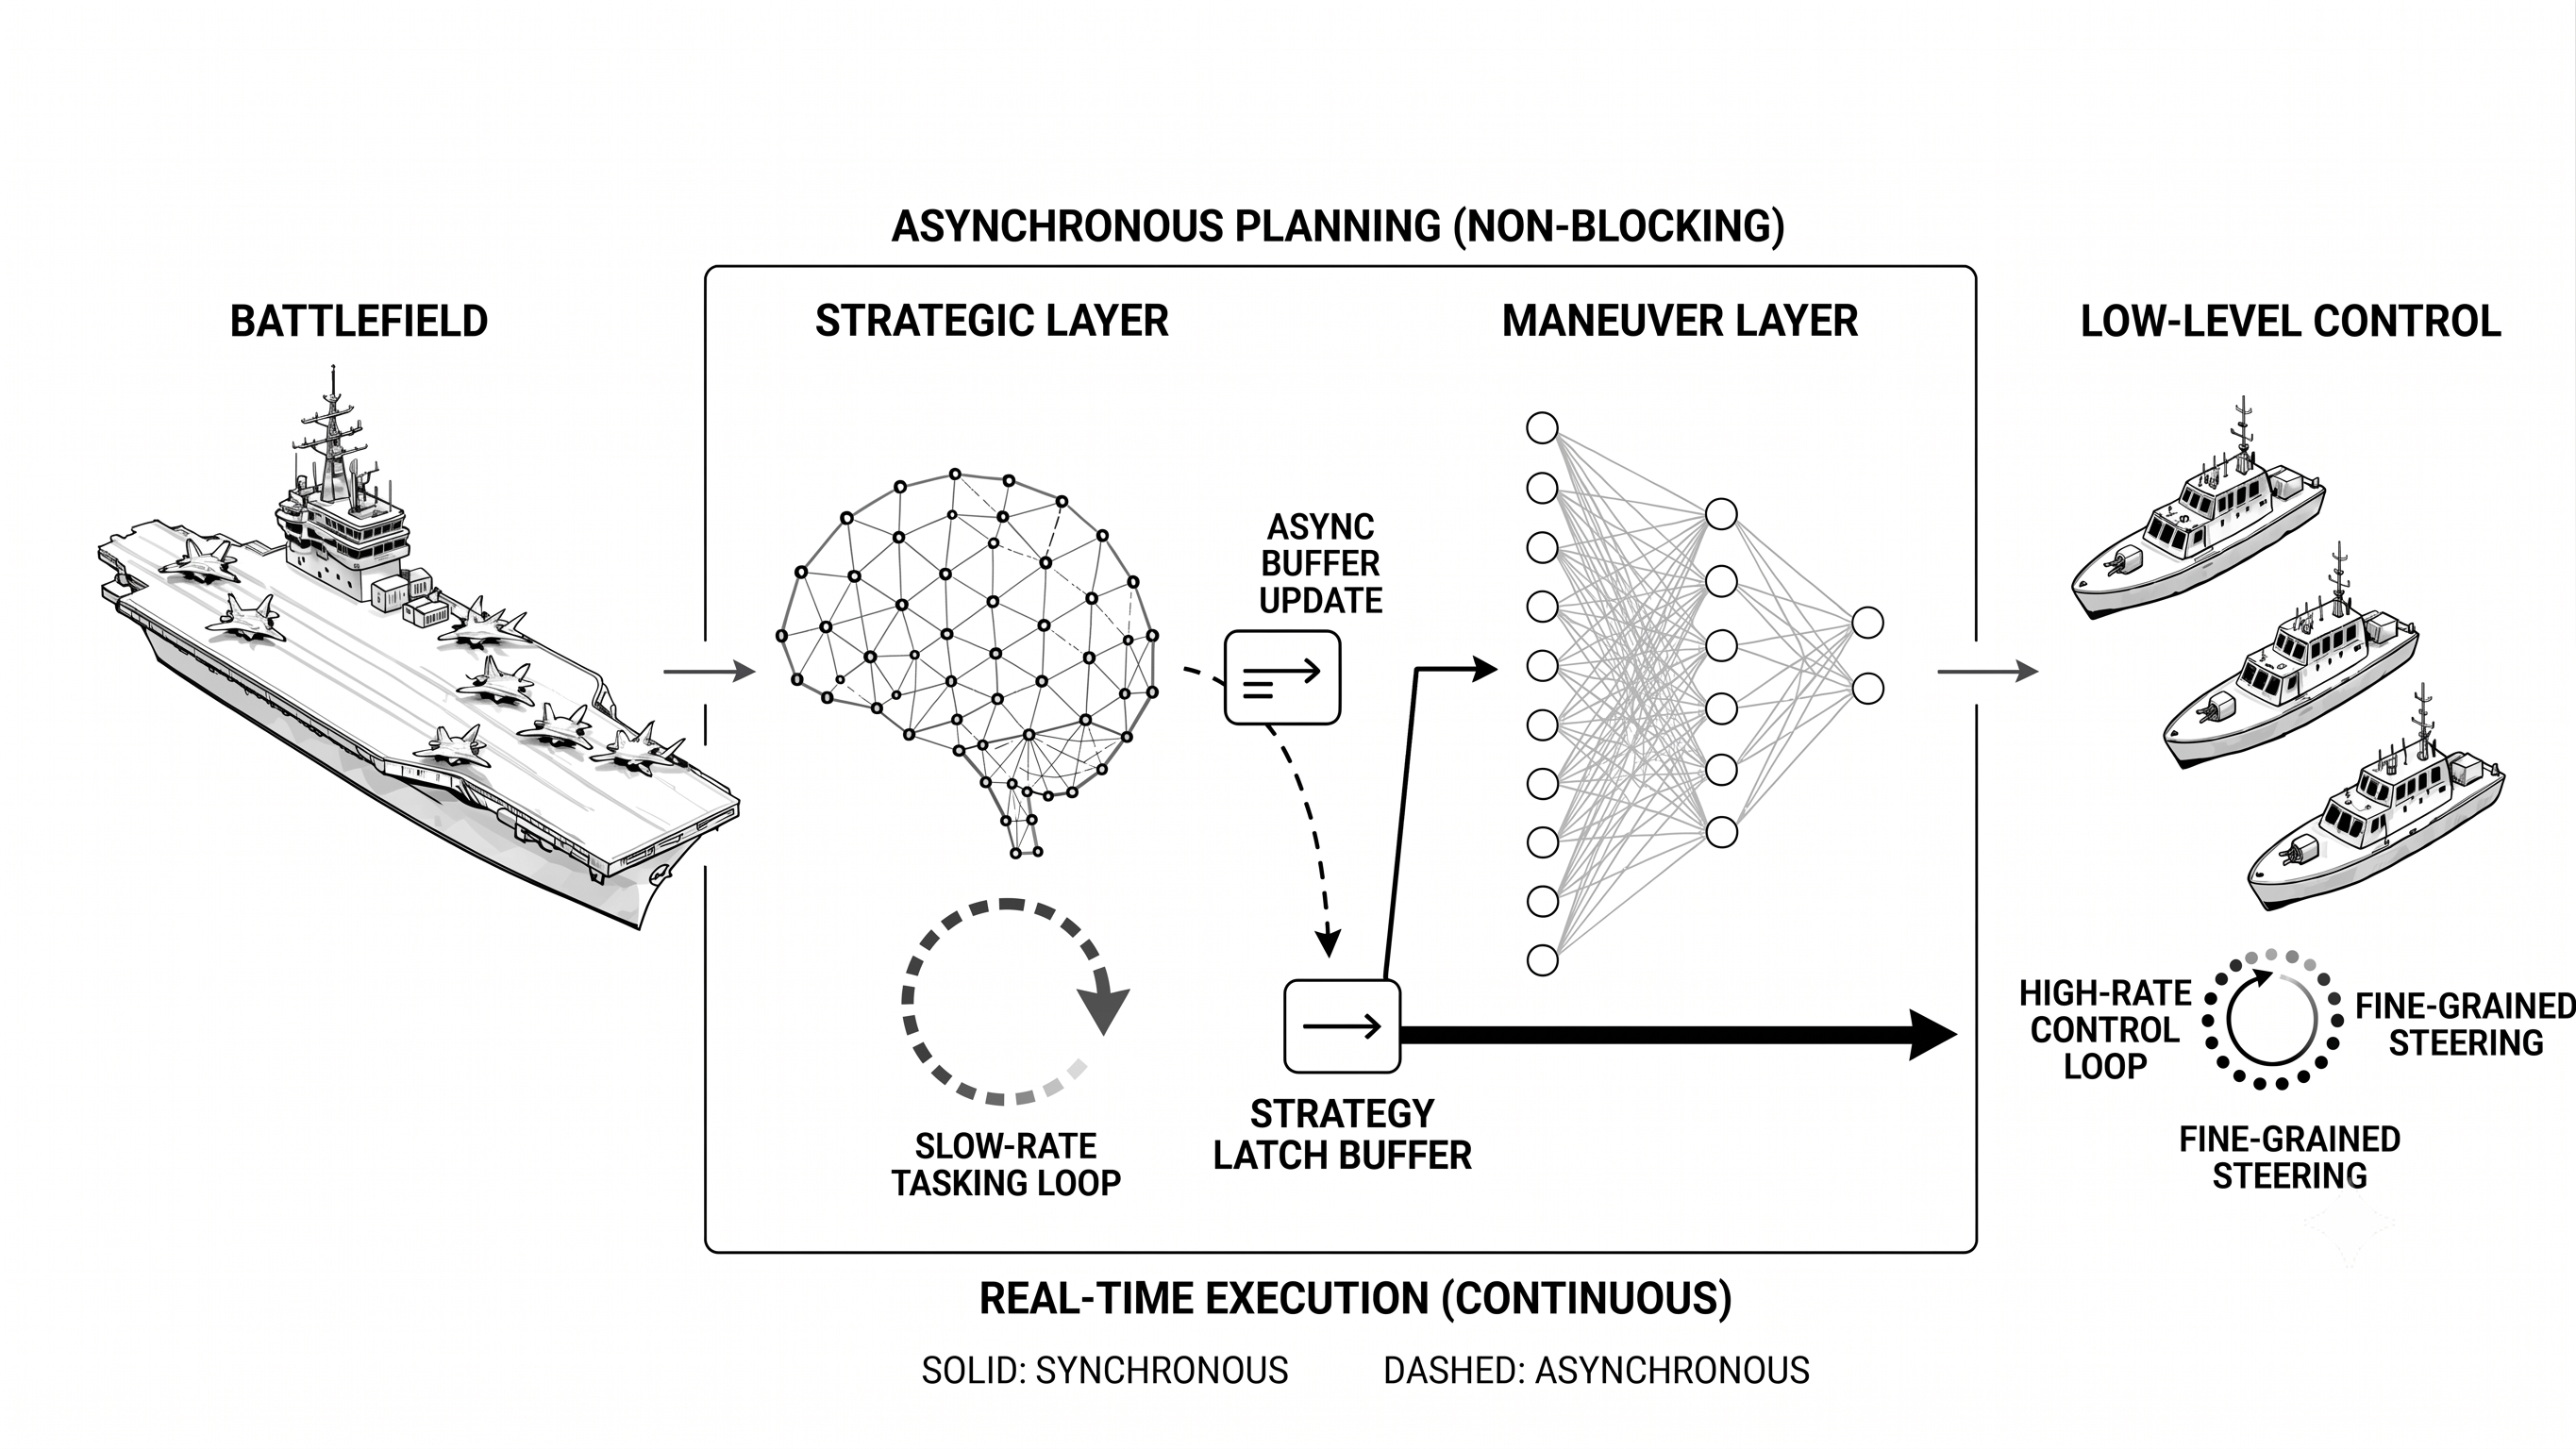
\includegraphics[width=0.72\textwidth]{fig4.png}
\caption{제안 체계의 2계층 구조}
\label{fig:architecture}
\end{figure*}

다수의 저비용 무인수상정(USV)이 고가치 함정을 향해 여러 방향에서 동시에 돌진하는 자폭
공격은 비대칭 위협의 전형이다. 유한한 방어 자산의 배분은 무기-표적 할당 문제로 오래
연구되었으나~\citep{ahuja2007wta}, 표적 수가 요격 자산을 넘어서면 최적 할당으로도 남는
표적이 생긴다. 교란에 의한 연성 대응(soft-kill)은 위협을 제거하지 못하고 유선 조종 표적에
무력하며~\citep{wang2021cuas, sutea2026fiber},
직접 타격하는 경성 대응(hard-kill)은 값싼 표적에 고가 유도탄을 쓰는 비용
구조~\citep{rumbaugh2024cost}와 표적 수에 따른 포화를 피하지 못한다.

본 연구는 저비용 그물에 의한 물리적 포획을 택한다~\citep{wang2021cuas}. 이 방식은 통신
방식과 무관하게 표적을 정지시킨다. 방어정은 적선보다 느려 추격할 수 없으므로, 적선이
지나갈 접근 회랑을 앞질러 그물벽으로 차단한다.

이 문제는 성격이 다른 두 판단을 요구한다. 하나는 어느 방어정이 어느 적 무리를 맡는가라는
이산적 배정이고, 다른 하나는 맡은 무리를 해면 어디에서 막는가라는 연속적 기동이다.
둘은 같은 주기로 갱신되지만 산출에 걸리는 시간이 크게 다르다. 본 연구는 느린 배정을
언어모델 지휘관에게, 빠른 기동을 학습된 정책에 맡기고 느린 계층만 비동기로
분리한다(Fig.~\ref{fig:architecture}).

학습과 평가는 OpenStreetMap 해안선을 래스터화한 실해역 지형에서 수행한다. 관측은 모선 중심
격자의 다채널 영상이고, 행동은 그 격자의 유효 픽셀 하나를 고르는 것이라 불가능한 자리가 애초에
뽑히지 않는다. 출력은 제어 신호가 아니라 경유점이라 저수준 추종과 분리된다(\ref{sec:method}절).
각 계층이 무엇을 얼마나 개선하는지는 시드 대응 $2\times2$ 설계로 분리해 측정한다
(\ref{sec:experiment}절).

%============================================================ 2. 관련 연구 (압축판)
%  원판의 5개 소절을 3개로 합치고, 계열 열거를 대표 문헌 한 줄로 줄였다.
\section{관련 연구}
\label{sec:related}

\subsection{자산 배분과 무인 위협 대응}

방어 자산을 표적에 배분하는 문제는 무기-표적 할당(WTA)으로 정식화되어 정확해법과
휴리스틱이 모두 연구되었고~\citep{ahuja2007wta}, 1:1 배정으로 축소하면 헝가리안
알고리즘~\citep{kuhn1955hungarian}으로 최소비용 매칭을 얻는다. 다만 이전 결정이 이미 막은
회랑과 남은 자산에 따라 달라지는 판단은 고정된 거리·각도 비용으로 표현되지 않는다. 본
연구는 배정 계층에 조합 최적화 대신 언어모델의 판단을 둔다.

무인 위협의 무력화 수단은 연성(전자전)·경성(물리 타격)·포획으로
구분되는데~\citep{wang2021cuas}, 유선 조종 표적의 확산~\citep{sutea2026fiber}이 연성의
범위를, 요격 비용의 비대칭~\citep{rumbaugh2024cost}이 경성의 지속성을 제약하면서 포획이
남는다. 해상에서는 다중 USV 협력 기동~\citep{liu2016usv}과 강화학습 협조
포위~\citep{zhang2025encircle}가 보고되었으나 포위는 방어정이 표적보다 빠르거나 대등함을
전제하므로, 더 느린 조건에서는 추격 대신 접근 경로의 선제 차단이 남는다.

\subsection{다중 에이전트 강화학습과 크레딧 배분}

중앙 집중 학습·분산 실행(CTDE) 계열은 팀 보상에서 개체별 기여를 분리하려고 가치망을
학습하며, 중앙 비평가~\citep{lowe2017maddpg}, 단조 가치 분해~\citep{rashid2018qmix},
반사실적 기준선~\citep{foerster2018coma}, PPO~\citep{schulman2017ppo}의 다중 에이전트
확장~\citep{yu2022mappo}이 그 예다. 그러나 공유 가치망의 추정 편향과 학습
불안정~\citep{haarnoja2018sac}은 여러 에이전트가 함께 학습하는 비정상 환경에서 더 커진다.
그룹 상대 정책 최적화(GRPO)~\citep{shao2024deepseekmath}는 같은 상태에서 뽑은 여러 후보의
보상을 서로 비교해 이득을 산정함으로써 가치망 자체를 없앤다. 본 연구는 GRPO를 다중 에이전트
제어로 옮기되, 후보 하나를 기하 휴리스틱으로 고정해 기준선으로 삼고 후보의 팀 보상을
비평가가 아니라 시뮬레이터 재진행으로 얻는다. 다중 에이전트 근위 정책 최적화(MAPPO)는
같은 픽셀 행동공간 위의
기준선으로 두어 표현과 갱신 규칙의 기여를 분리한다(\ref{sec:res_algo}절).

\subsection{격자 표현·픽셀 지목과 언어모델 계획}
% Fig.2 는 §3.1 보다 먼저 보여야 한다. 2단 figure* 는 만난 쪽의 다음 쪽 상단에 놓이므로
% §3 이 시작하는 쪽 상단에 오도록 그 앞 쪽의 이 자리에서 선언한다.
\begin{figure*}[!t]
\centering
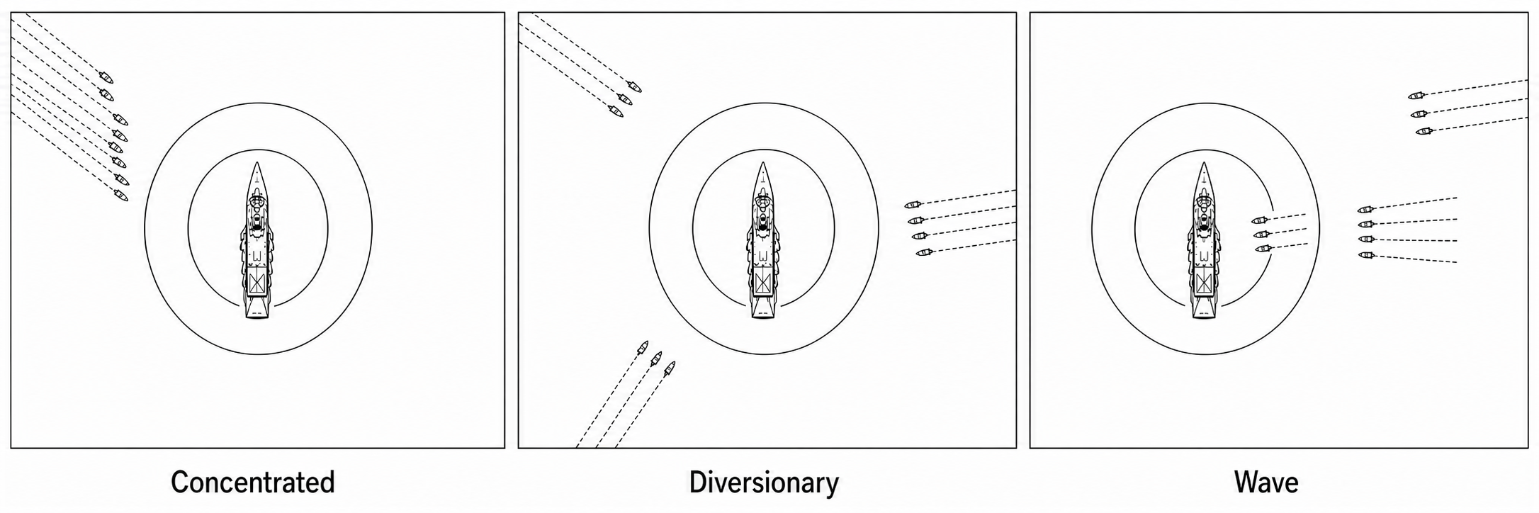
\includegraphics[width=\textwidth]{fig2.png}
\caption{세 가지 공격 포메이션: 집중·양동·파상(좌$\to$우)}
\label{fig:formations}
\end{figure*}

모든 픽셀에 값을 매기는 조밀 예측 계열~\citep{long2015fcn, ronneberger2015unet}과 그 확장인
좌표 채널~\citep{liu2018coordconv}·조건 변조~\citep{perez2018film}는 모두 상황 지각에
쓰였고, 후보마다 점수를 매겨 하나를 지목하는 출력~\citep{vinyals2015pointer,
vaswani2017attention}은 주로 조합 최적화에 머물렀다. 본 연구는 둘을 잇는다. U-Net 특징
지도의 각 픽셀에 방어정별 질의로 점수를 매기고(\ref{sec:policy}절), 그 점수맵을 정책의
행동 분포로 삼아 픽셀 하나를 지목하는 것이 곧 행동이므로, 안전 제약을 마스크로 행동 분포에
직접 부과할 수 있다.

언어모델을 계획 주체로 쓰는 연구는 고수준 지시를 실행 가능한 단계로
분해하고~\citep{huang2022zeroshot}, 실행 가능성 추정을 결합해 불가능한 계획을
걸러내며~\citep{ahn2022saycan}, 구조적 출력~\citep{openai2026function}으로 하위 시스템이 파싱
가능한 형태를 보장한다. 본 연구도 판단을 실행 가능성으로 거르되, 언어모델에는 배정만 맡기고
실행 가능성은 기동 계층의 유효 마스크가 픽셀 수준에서 강제한다(\ref{sec:validmask}절).

%============================================================ 3. 문제 정의 (압축판)
\section{문제 정의와 평가 지표}
\label{sec:problem}

\subsection{교전 시나리오}
\label{sec:scenario}
%============================================================ 교전 시나리오 표 (국방발표 판)
%  저널판은 tables/tab_scenario.tex(자동 생성)를 쓰고 길이를 관측 픽셀 한 변 $\ell$ 단위로
%  적는다. 발표판은 같은 설정을 m·m/s 로 환산해 싣는다 --- 환산 기준은 기준 인스턴스
%  $\ell = 252\unit{m}$, 결정 주기 25\,s 이며, 원값은 학습 체크포인트의 설정이다.
%    교전 해역 한 변 50 \ell = 12.6 km,  적 0.89 \ell/주기 = 9.0 m/s,  방어정 0.60 \ell/주기 = 6.0 m/s
%  표 밑 주석은 싣지 않는다(발표판 방침).
\begin{table}[htbp]
\centering
\caption{교전 시나리오와 관측 설정}
\label{tab:scenario}
\footnotesize
\resizebox{\ifdim\width>\linewidth\linewidth\else\width\fi}{!}{%
\begin{tabular}{lr}
\toprule
항목 & 값 \\
\midrule
적 USV 수 $M$ & 10 \\
방어정 수 $P$ & 3 \\
적 무리 최대 수 $C$ & 4 \\
교전 해역 한 변 & $12.6\unit{km}$ \\
적 USV 속력 $v_e$ & $9.0\unit{m/s}$ \\
방어정 속력 $v_a$ (속력비 $v_e/v_a = 1.5$) & $6.0\unit{m/s}$ \\
결정 주기 & $25\unit{s}$ \\
관측 격자 $n_{\mathrm{g}} \times n_{\mathrm{g}}$ (모선 중심) & $50 \times 50$ \\
관측 픽셀 한 변 $\ell$ & $252\unit{m}$ \\
방어정당 그물 (학습 / 평가) & 1 / 3 \\
정책 파라미터 수 & 244{,}389 \\
\bottomrule
\end{tabular}
}
\end{table}


\begin{table*}[!b]
\centering
\caption{평가 지표 10종(화살표는 개선 방향)}
\label{tab:metrics}
\footnotesize
\renewcommand{\arraystretch}{1.25}
\begin{tabular}{llcp{0.27\linewidth}p{0.37\linewidth}}
\toprule
관점 & 지표 & 방향 & 정의 & 뜻 \\
\midrule
\multirow{2}{*}{방어 성과}
 & 포획률           & $\uparrow$   & $\capr = N_\mathrm{cap} / (N_\mathrm{cap} + N_\mathrm{brc})$ & 교전이 결판난 적선 중 포획된 비율 \\
 & 돌파 수          & $\downarrow$ & $N_\mathrm{brc}$ & 모선까지 도달한 적선 수 \\
\midrule
\multirow{2}{*}{안전}
 & 충돌률           & $\downarrow$ & $N_\mathrm{col} / P$ & 방어정 1척당 아군 상호·모선 충돌 건수 \\
 & 그물 걸림        & $\downarrow$ & $N_\mathrm{tng}$ & 아군이 설치된 그물에 얽힌 횟수 \\
\midrule
\multirow{2}{*}{자원 효율}
 & 포획당 그물      & $\downarrow$ & $N_\mathrm{net} / N_\mathrm{cap}$ & 적 1척 포획에 소모한 그물 수 \\
 & 포획당 이동거리  & $\downarrow$ & $\sum_{p=1}^{P} D_p \,/\, N_\mathrm{cap}$ & 적 1척 포획당 팀 총 이동거리 \\
\midrule
기동 비용
 & 총 선회량        & $\downarrow$ & $\sum_{p=1}^{P} \sum_{t} \lvert \Delta\psi_{p,t} \rvert$ & 누적 방위 변화량(궤적 부드러움) \\
\midrule
\multirow{3}{*}{교전 품질}
 & 포획 이격거리    & $\uparrow$   & $\frac{1}{N_\mathrm{cap}} \sum_{k} \lVert \mathbf{z}_k - \mathbf{m} \rVert$ & 포획 지점의 모선 이격(공간축 조기 제압) \\
 & 평균 포획 시각   & $\downarrow$ & $\frac{1}{N_\mathrm{cap}} \sum_{k} t_k$ & 포획이 일어난 시각(시간축 조기 제압) \\
 & 전개 시 적 거리  & $\downarrow$ & $\frac{1}{N_\mathrm{net}} \sum_{d} \min_{m \in \mathcal{A}} \lVert \mathbf{a}_d - \mathbf{e}_m \rVert$ & 그물 전개를 시작한 순간 최근접 적까지 거리 \\
\bottomrule
\end{tabular}
\end{table*}

교전 해역 중앙에 고가치 모선 한 척이 있고, 가장자리에서 적 USV $M$척이 모선을 향해
돌진한다. 적은 집중·양동·파상의 세 공격 포메이션 가운데 하나를
취한다(Fig.~\ref{fig:formations}). 방어정 $P$척은 각각 한정된 수의 그물벽을 전개할 수
있다. 체계는 스케일 불변이므로 아래는 한 기준 인스턴스다. 교전 해역은 한 변
$12.6\unit{km}$ 의 정사각 해역이고, 적선은 $9.0\unit{m/s}$, 방어정은
$6.0\unit{m/s}$ 로 적이 1.5배 빠르며, 두 계층 모두 $25\unit{s}$ 마다 결정한다
(Table~\ref{tab:scenario}). 관측·행동·보상은 모두 관측 픽셀 한 변 $\ell = 252\unit{m}$ 로
정규화한다(\ref{sec:obs}절).

방어정은 적이 지나갈 자리를 미리 선점해야 한다. 그물벽은 두 좌표를 잇는 선분이고, 방어정이
그 선분을 따라 이동하면서 후미의 전개 장치로 부유식 그물을 해면에 풀어 놓는다. 그 위를 지나는
적 USV가 추진을 잃는 것을 포획으로 본다(Fig.~\ref{fig:netconcept}). 전개된 그물은 해면에
고정되지 않아 시간이 지날수록 차단 효과가 줄고, 미리 전개하면 적에게 노출되어 회피의 여지를
준다. 그물벽을 적의 도달 직전, 적에 가까운 위치에 두는 것이 유리하다고 가정한다.

\begin{figure}[!htbp]
\centering
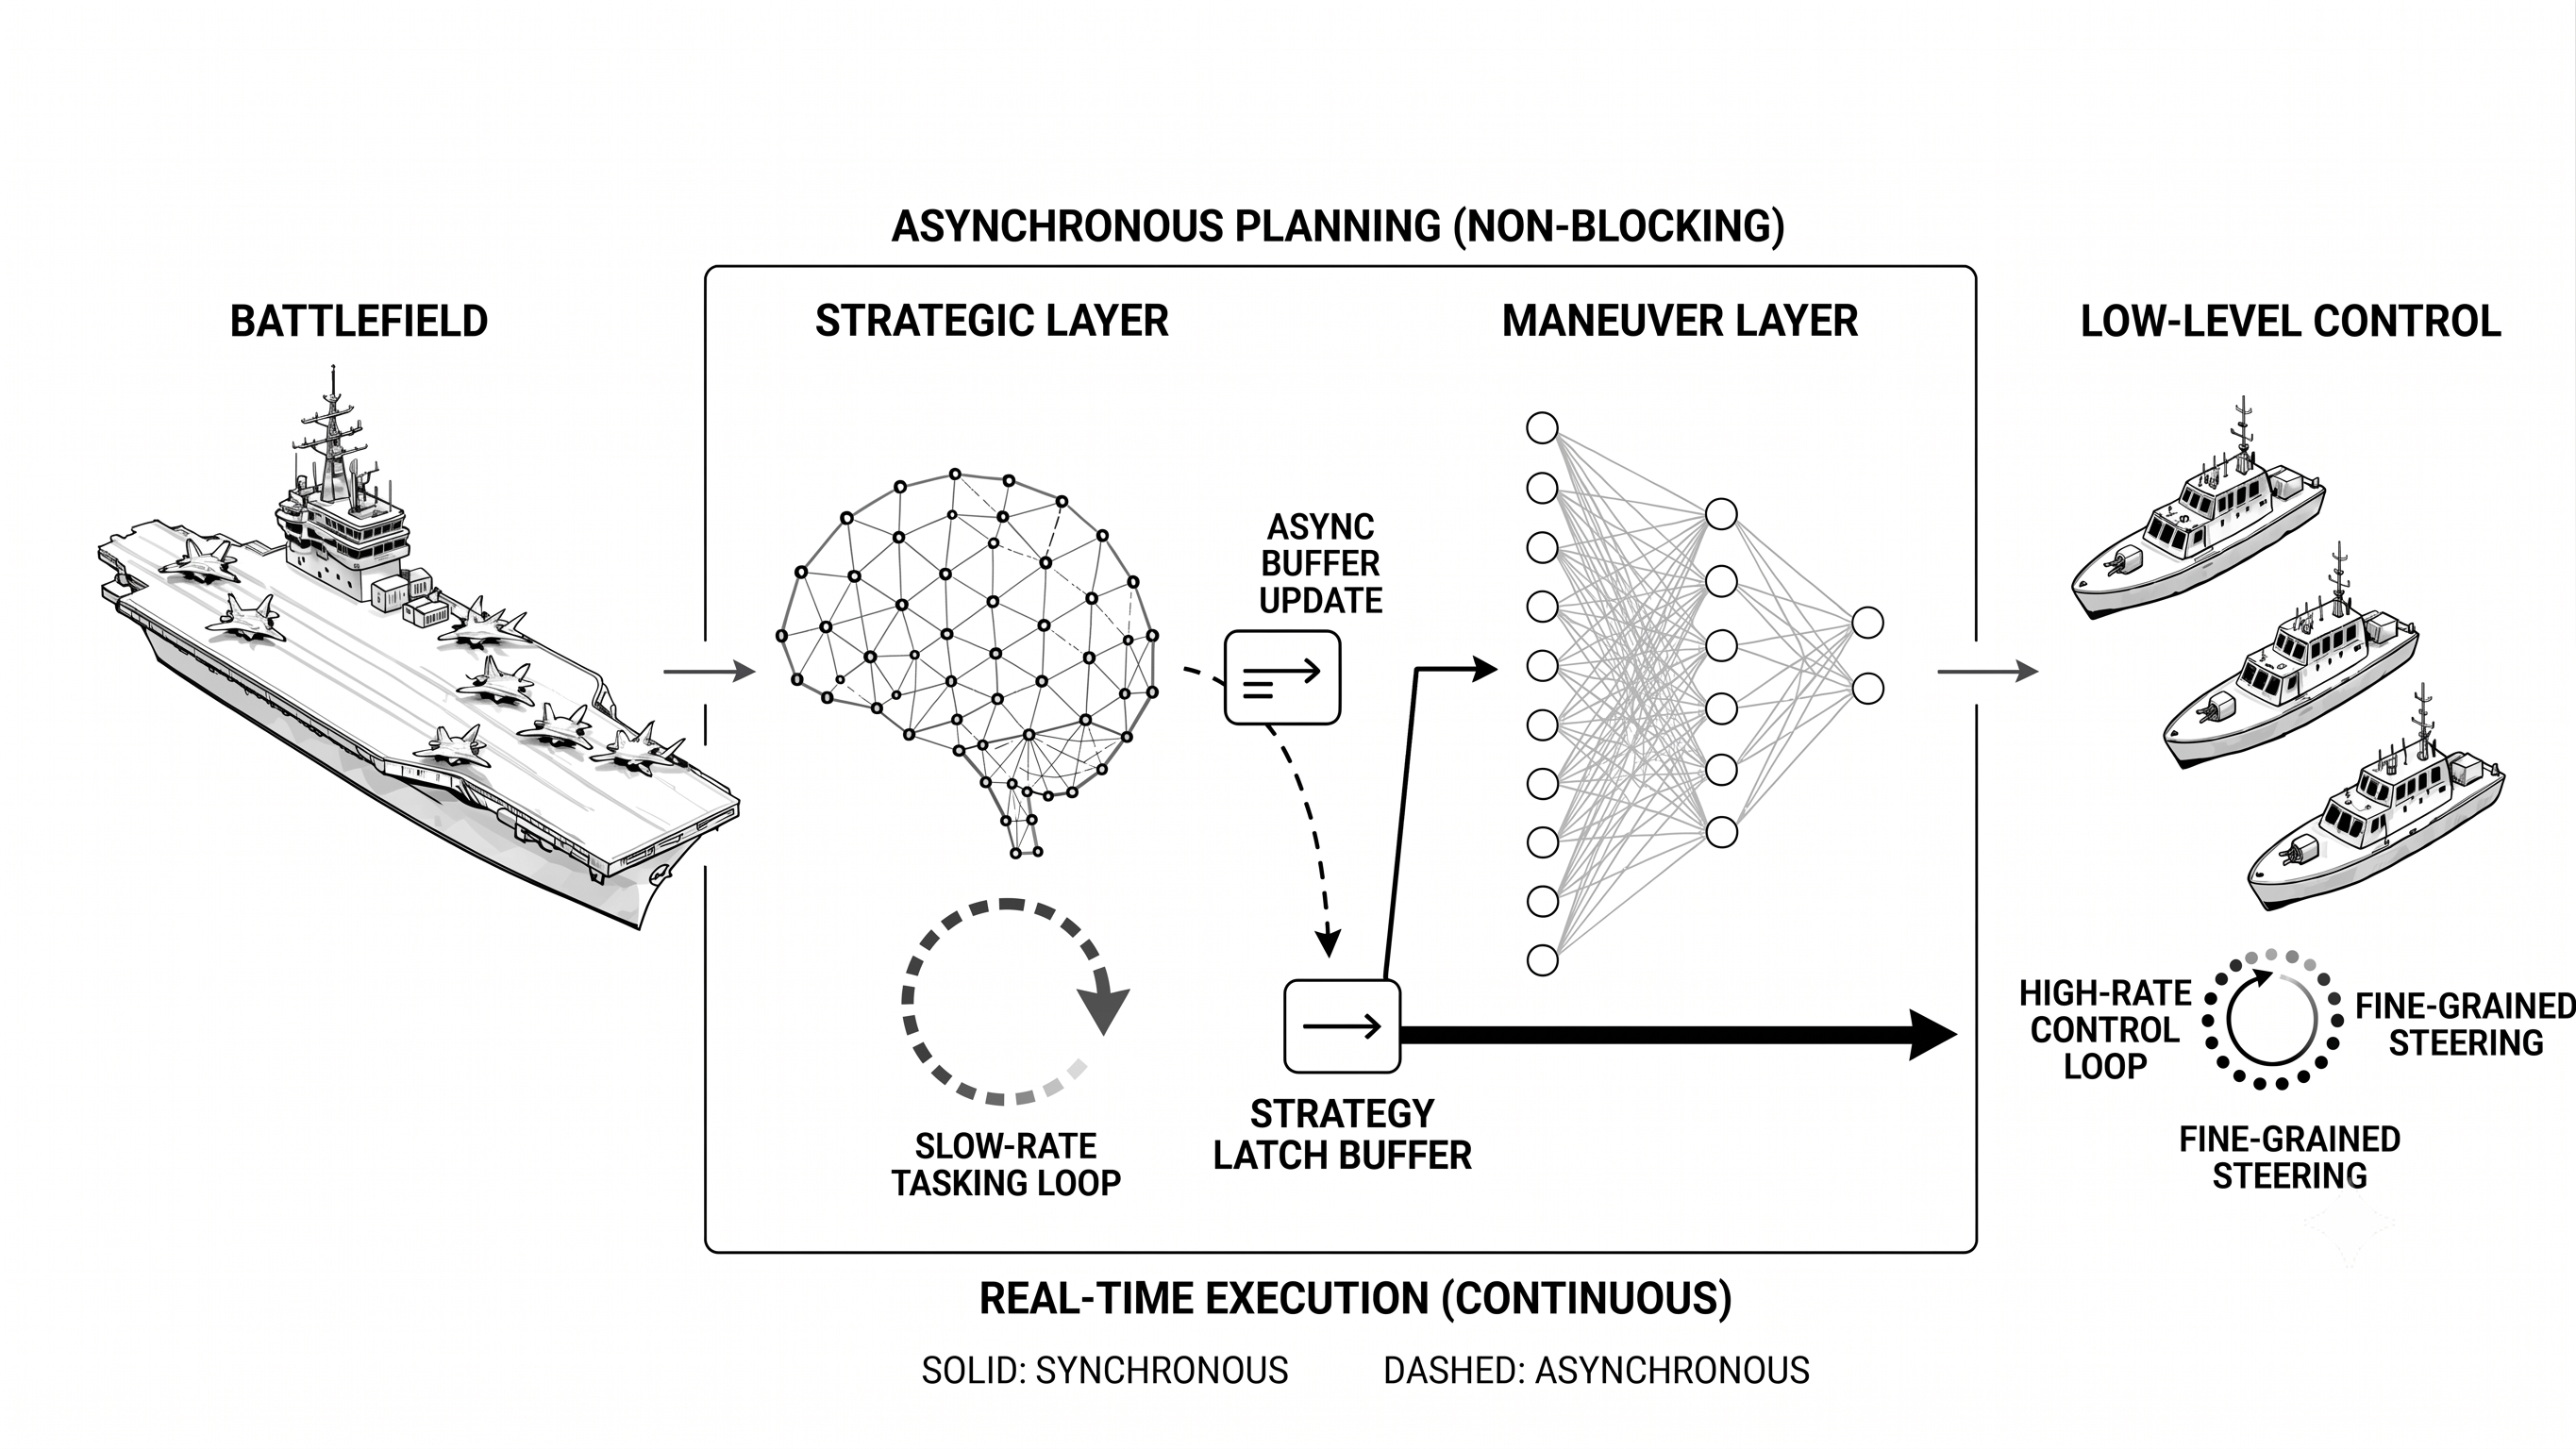
\includegraphics[width=0.62\columnwidth]{fig3.png}
\caption{후미 투하식 부유 그물의 포획 개념}
\label{fig:netconcept}
\end{figure}

\begin{itemize}[leftmargin=*, itemsep=3pt, topsep=3pt]
\item 집중(concentrated): 적 전 병력이 한 방위에서 동시에 접근한다. 차단할
      접근로가 하나라 소수의 방어정으로도 대응된다.
\item 양동(diversionary): 적이 세 방위로 나뉘어 동시에 접근한다. 가용 방어정을 모두
      투입해야 하므로 어느 배가 어느 무리를 맡는 배정이 결과를 좌우한다.
\item 파상(wave): 적이 3개 단(rank)으로 나뉘어 방위를 조금씩 달리하며 거리차를 두고
      순차 도달한다. 앞 단에 쓴 그물벽은 그 자리에 남고 보유량은 한정되므로, 그물벽을
      어느 자리에 놓아 여러 단을 겸해 막을지가 관건이다.
\end{itemize}

\subsection{평가 지표}
\label{sec:metrics}

방어 성과는 다섯 관점의 10개 지표로 에피소드마다 잰다(Table~\ref{tab:metrics}). 자원 효율은
교전하지 않은 조건이 가장 효율적으로 보이는 것을 막기 위해 총량이 아니라 포획당 비율로
두었고, 교전 품질은 거리축과 시간축으로 나누어 모선에서 먼 포획과 이른 포획을 함께 본다.

% 기호표(Table, tab:nomenclature): §4.1 첫 문단이 참조한다. 2단 table* 는 선언된 쪽에
% 놓일 수 없어 §4 안에서 선언하면 한 쪽 뒤로 밀리므로, §3 끝(앞 쪽 본문)에서 선언해
% §4 가 시작하는 쪽 하단([!b])에 앉힌다.
%% 기호표는 발표판에서 싣지 않는다 --- 각 기호를 본문 첫 등장 자리에서 정의한다.
%% %============================================================ 제안 체계의 기호표 (압축판)
%  §4 가 산문화되면서 사라진 기호를 솎아냈다. 표에만 있고 본문에 없는 기호는 독자를 찾아
%  헤매게 만들므로, 기호를 더하려면 본문에 실제로 그 기호가 있는지 먼저 확인할 것.
\begin{table*}[tp]
\caption{제안 체계(\ref{sec:method}절)의 기호}
\label{tab:nomenclature}
\centering\footnotesize
\resizebox{\ifdim\width>\linewidth\linewidth\else\width\fi}{!}{%
\begin{tabular}{@{}ll@{\hspace{1.6em}}ll@{}}
\toprule
\textbf{기호} & \textbf{뜻} & \textbf{기호} & \textbf{뜻} \\
\midrule
$A_k$                 & 후보 $k$ 의 그룹 상대 이득           & $r_{\mathrm{dup}}$      & 경유점 중복 배제 반경 \\
$\mathbf{a}_p$        & 방어정 $p$ 의 위치                & $s_{p,i}$               & 방어정 $p$ 가 픽셀 $i$ 에 준 점수 \\
$C$, $\hat{C}$        & 무리 수 상한, 활성 무리 수            & $\mathbf{t}_k$          & $k$ 번째 목표점 (연속 좌표) \\
$\mathbf{c}_j$, $n_j$ & 무리 $j$ 의 중심, 척수             & $\mathcal{V}_p$         & 방어정 $p$ 의 유효 픽셀 집합 \\
$d_{pj}$              & 방어정 $p$ $\to$ 무리 $j$ 요격점 거리 & $w_n$                   & 유효 월드 마스크 \\
$E$, $\ell$           & 관측 반폭, 픽셀 크기                & $\mathbf{x}_i$          & 픽셀 $i$ 의 중심 좌표 \\
$\mathbf{f}_i$        & 픽셀 $i$ 의 키 벡터               & $\beta$                 & 배정 유지 보너스 (식~\ref{eq:sticky}) \\
$G$                   & 학습의 그룹 후보 수                 & $\gamma$                & 퍼텐셜 성형 할인 계수 \\
$g_{(q)}$             & 정렬한 적선 방위의 $q$ 번째 간격        & $\delta_{\mathrm{gap}}$ & 무리 분할 방위 임계 \\
$H$                   & 후보 평가 창 길이                  & $\vartheta_m$           & 모선에서 본 적선 $m$ 의 방위 \\
$\mathbf{I}$          & 요격점                         & $(\iota_x, \iota_y)$    & 월드 $\to$ 픽셀 인덱스 (식~\ref{eq:world2pix}) \\
$K$                   & 방어정 1척이 지목하는 경유점 수          & $\lambda_{\mathrm{I}}$  & 요격점의 모선 쪽 치우침 비율 \\
$L_{\mathrm{net}}$    & 그물벽 최대 길이                   & $\lambda_{\mathrm{L}}$  & 잉여 방어정의 층 분리 증분 \\
$M$                   & 적 USV 수                     & $\tau_j$                & 무리 $j$ 의 위협도 \\
$n_{\max}$            & 방어정 1척당 그물 보유량              & $\Phi$                  & 위협 근접도 퍼텐셜 \\
$\mathbf{o}_p$        & 방어정 $p$ 의 자체 상태 벡터          & $R_k$                   & 후보 $k$ 의 팀 보상 \\
$P$                   & 방어정 수                       & $R_w$                   & 교전 해역 반폭 \\
$\mathbf{q}_p$        & 방어정 $p$ 의 질의 벡터             &                         &  \\
\bottomrule
\end{tabular}}
\end{table*}

%============================================================ 4. 제안 방법 (압축판)
%  원판(sections_real/04_method.tex)에서 구현 세부 수식을 산문으로 내리고, 결과에 쓰이지
%  않은 반사실 크레딧 변형을 덜어냈다. 남긴 식은 방법의 정체성을 정하는 것들이다.
\section{제안 방법}
\label{sec:method}

\subsection{2계층 비동기 구조}
\label{sec:arch}

제안 체계는 방어 판단을 전략 계층과 기동 계층으로 분리한다(Fig.~\ref{fig:architecture}).
전략 계층은 어느 방어정이 어느 적 무리를 맡는가를 정하고, 기동 계층은 배정된
무리를 막기 위해 해면 어디에 그물벽을 놓는가를 정한다. 두 계층은 같은 주기로 결정을
내리지만 응답 속도가 다르다. 기동 계층의 순전파는 순간에 끝나는 반면, 전략 계층의
언어모델 호출은 응답에 지연이 발생한다(\ref{sec:res_latency}절). 느린 전략 계층 호출만
비동기로 분리하여, 호출이 진행되는 동안 기동 계층은 직전 배정으로 결정을 계속하고 응답이
도착하면 다음 결정부터 새 배정을 반영한다.

\subsection{적 무리 군집화}
\label{sec:cluster}
\begin{figure}[!htbp]
\centering
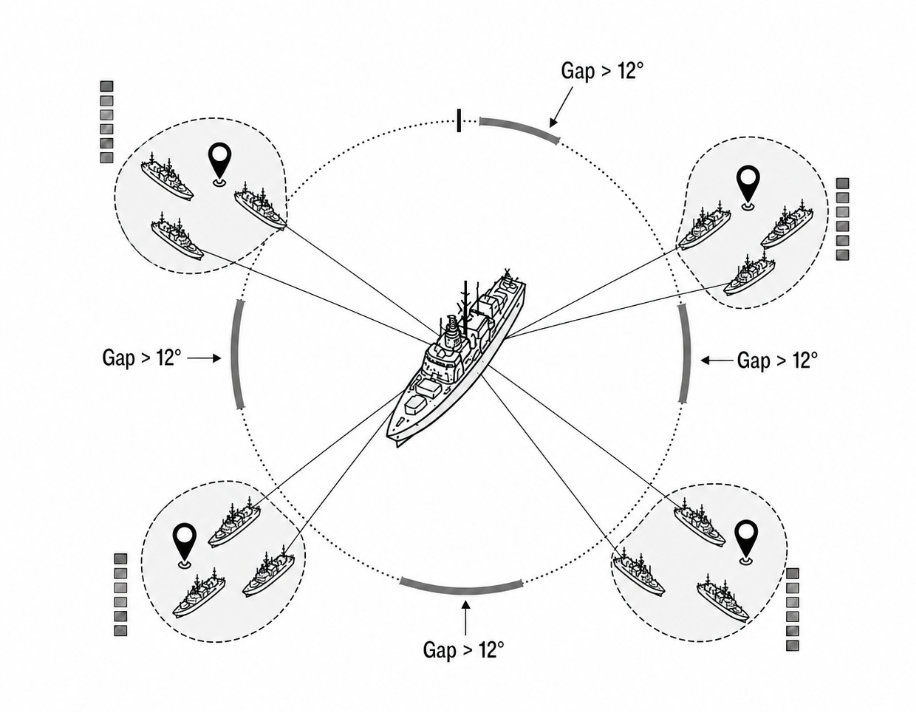
\includegraphics[width=\columnwidth]{fig5.png}
\caption{방위각 정렬, 군집화, 군집 배정}
\label{fig:clustering}
\end{figure}

두 판단 계층은 개별 적선이 아니라 무리를 단위로 배정하므로, 매 결정마다 생존 적선을 모선
기준 방위 $\vartheta_m$ 으로 묶어 최대 $C$ 개의 무리로 요약한다(Fig.~\ref{fig:clustering}).
방위 구간을 고정해 나누면 무리가 경계에 걸려 쪼개지므로, 정렬한 방위의 이웃 간격 $g_{(q)}$ 로
무리 수를 데이터에 맞춘다. 방위는 순환값이라 간격도 순환으로 센다. 임계
$\delta_{\mathrm{gap}}$ 을 넘는 간격의 개수가 활성 무리 수 $\hat{C}$ 이며,
$1$ 이상 $\min(C, n)$ 이하로 자른다.
\begin{equation}
\hat{C} = \mathrm{clip}\!\Big(\big|\{\, q : g_{(q)} > \delta_{\mathrm{gap}} \,\}\big|,\; 1,\; \min(C, n)\Big)
\label{eq:ncluster}
\end{equation}
가장 큰 간격 $\hat{C}$ 개를 경계로 삼아 방위 순으로 라벨을 붙여 무리별 구성원을 정하고, 각
무리를 척수 $n_j$, 중심 $\mathbf{c}_j$, 각도 퍼짐 $\Delta\vartheta_j$, 모선 방향 접근 속도
$v^{\mathrm{app}}_j$ 의 네 양으로 요약한다.
% ★ Fig.6(fig:observation) 은 2단 figure* 라 선언된 쪽에 놓일 수 없어 여기(§4.2 끝)에서
%   선언해야 §4.4.1 이 시작하는 쪽 상단에 앉는다.
\begin{figure*}[!tp]
\centering
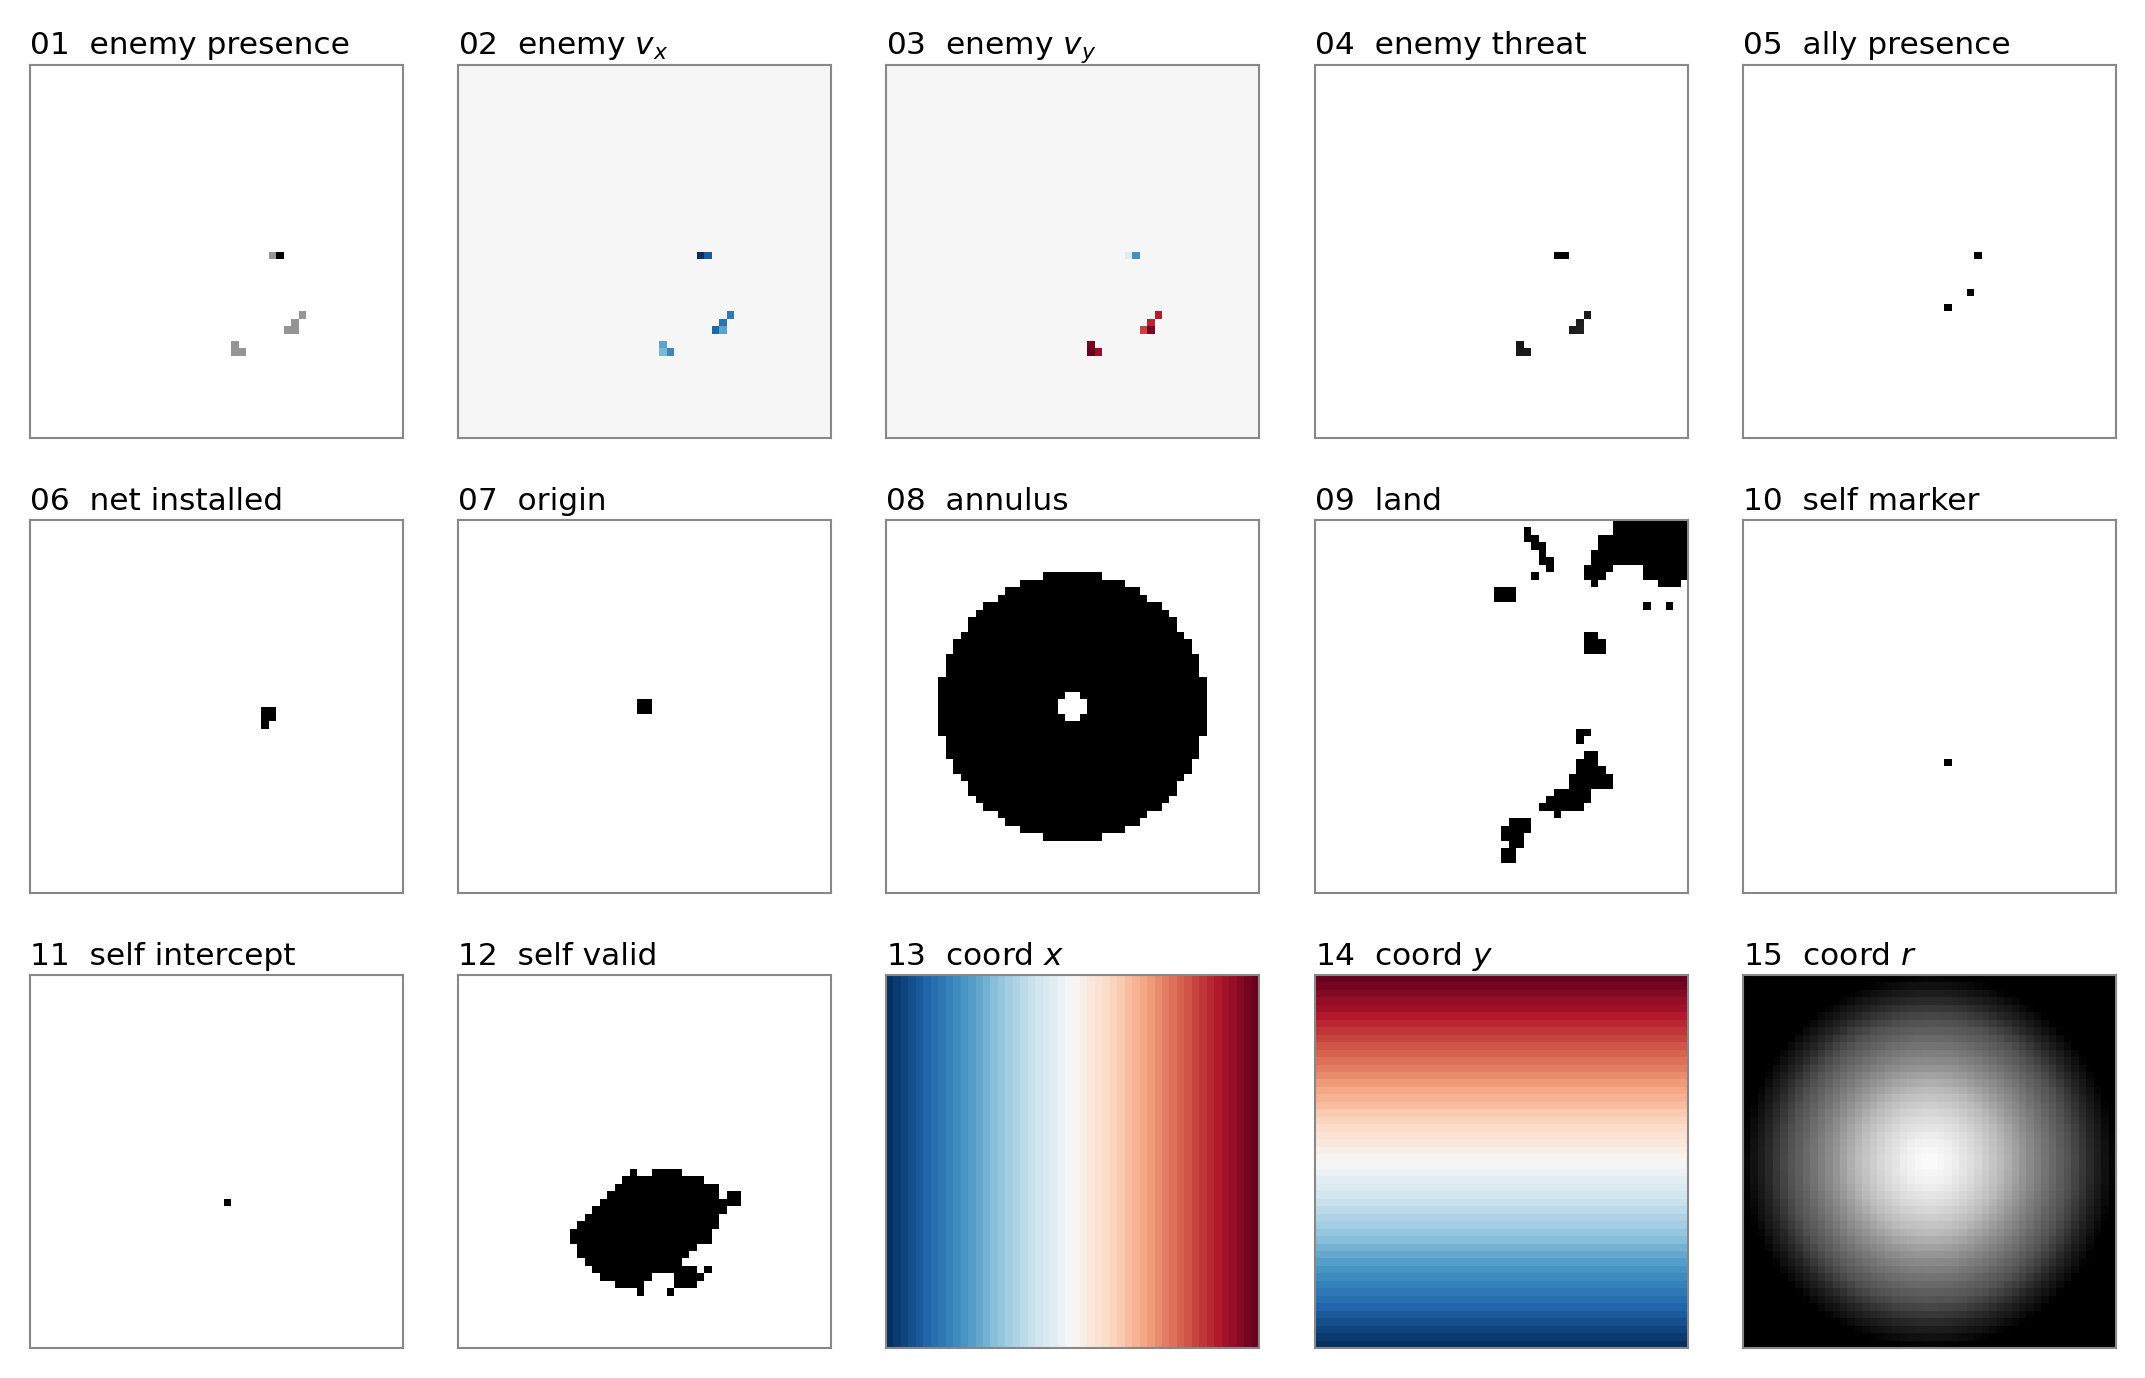
\includegraphics[width=0.62\textwidth]{fig6.png}
\caption{래스터화된 15채널 관측의 예(파상, 통영 매물도 북측)}
\label{fig:observation}
\end{figure*}

이 규칙에서 집중은 무리 하나, 양동은 셋, 파상은 대개 단마다 하나로 요약된다. 척수와 중심은
\ref{sec:heuristic}절의 위협도와 요격점을, 네 요약량 전부는 \ref{sec:commander}절의
지휘관 입력을 구성한다.

\subsection{기하 휴리스틱 기준 방법}
\label{sec:heuristic}

무리 요약 위에서 같은 문제를 기하 규칙만으로 푸는 기준 방법으로, \ref{sec:results}절의 비교
기준이자 \ref{sec:bc}절의 행동 복제 목표다. 무리 $j$ 의 위협도 $\tau_j$ 는 척수 $n_j$ 에 모선
근접도를 곱한 양이고, 요격점 $\mathbf{I}_j$ 는 무리 중심에서 모선을 향해 선분의 $\lambda_{\mathrm{I}}$
비율만큼 옮긴 점이다.
\begin{equation}
\begin{aligned}
\tau_j &= n_j \cdot \mathrm{clip}\!\left(1 - \frac{\lVert \mathbf{c}_j - \mathbf{m}\rVert}{R_w},
         \, 0.05,\, 1\right),\\
\mathbf{I}_j &= \mathbf{c}_j + \lambda_{\mathrm{I}}\,(\mathbf{m} - \mathbf{c}_j), \qquad \lambda_{\mathrm{I}} = 0.55
\end{aligned}
\label{eq:threat}
\end{equation}
하한은 먼 무리도 척수에 비례하는 최소 위협을 갖게 한다. 방어정이 적보다 느려 무리 중심
가까이 잡은 요격점에는 적보다 늦게 도달하므로, 요격점은 모선 쪽으로 치우쳐 둔다.

위협 상위 $P$ 개 무리에 대해 탐욕적 1:1 배정을 한다. 비용은 방어정 위치 $\mathbf{a}_p$ 에서
요격점까지의 거리 $d_{pj}$ 에서, 직전 결정의 담당 $j_p^{\text{prev}}$ 를 유지하는 쌍에만
보너스 $\beta$ 를 감한 값이다. $\beta$ 는 해역 규모에 맞먹는 크기로 두어, 거리 차이가
그만큼 벌어지기 전에는 직전 배정이 유지되게 한다.
\begin{equation}
\tilde{d}_{pj} = \begin{cases}
  d_{pj} - \beta, & j = j_p^{\text{prev}}\\
  d_{pj},          & \text{그 밖}
\end{cases}
\label{eq:sticky}
\end{equation}
활성 무리가 $P$ 보다 적으면 남는 방어정은 부하가 가장 큰 무리에 안쪽 층으로 덧붙인다. 층은 반경 증분 $\lambda_{\mathrm{L}}$ 과 방위차만큼 어긋나게 둔다. 그물벽은 요격점을 가운데 둔, 접근 방향에 수직인
길이 $L_{\mathrm{net}}$ 의 선분이므로 경유점은 그 양 끝 $K = 2$ 개이며, 학습 정책과 같은
격자·유효 마스크(\ref{sec:validmask}절) 위의 최근접 픽셀로 스냅한다.

따라서 두 방법의 행동공간은 같고 다른 것은 결정 규칙뿐이다.

\subsection{점수맵 기반 기동 정책}
\label{sec:policy}

\subsubsection{다채널 격자 관측}
\label{sec:obs}

기동 계층의 입력은 좌표 목록이 아니라, 모선을 중앙에 두고 관측 반폭 $E$ 의 전장을
$n_{\mathrm{g}} \times n_{\mathrm{g}}$ 격자로 나눈 다채널 지도이다. 총 15개 채널은 모든
방어정이 공유하는 전역 9채널, 방어정마다 다른 3채널, CoordConv~\citep{liu2018coordconv}
좌표 3채널로 구성되며(Fig.~\ref{fig:observation}), 각 채널의 정의와 값 범위를
Table~\ref{tab:channels}에 정리하였다.

\begin{table*}[!tp]
\centering
\caption{15채널 격자 관측의 구성}
\label{tab:channels}
\footnotesize
\renewcommand{\arraystretch}{1.15}
\begin{tabular}{@{}clllc@{}}
\toprule
\# & 묶음 & 채널 & 정의 & 범위 \\
\midrule
1  & \multirow{9}{*}{전역}   & 적 밀도        & 픽셀 내 생존 적선 수$/M$                                & $[0,1]$ \\
2  &                         & 적 진행 $x$    & 픽셀 내 적선 헤딩 단위벡터의 평균                      & $[-1,1]$ \\
3  &                         & 적 진행 $y$    & 위와 같음                                              & $[-1,1]$ \\
4  &                         & 적 위협도      & 모선 도달 임박도의 픽셀 내 최대                        & $[0,1]$ \\
5  &                         & 아군 위치      & 픽셀 내 생존 방어정 수$/P$                             & $[0,1]$ \\
6  &                         & 설치된 그물    & 물리 격자의 그물 점유를 최대값 풀링                     & $\{0,1\}$ \\
7  &                         & 원점           & 모선 반경 안의 픽셀                                    & $\{0,1\}$ \\
8  &                         & 요격 구역      & $r_{\min} \le \lVert \mathbf{x}_i - \mathbf{m} \rVert \le r_{\max}$ 인 픽셀 & $\{0,1\}$ \\
9  &                         & 육지           & 고해상도 육지 마스크의 면적비  & $[0,1]$ \\
\midrule
10 & \multirow{3}{*}{방어정별} & 자기 위치     & 방어정 $p$ 가 놓인 픽셀                                & $\{0,1\}$ \\
11 &                         & 배정 요격점    & $\mathbf{I}_p$ 가 놓인 픽셀 (미배정이면 전부 0)        & $\{0,1\}$ \\
12 &                         & 유효 영역      & 유효 마스크 $\mathcal{V}_p$, 식~\eqref{eq:validset}    & $\{0,1\}$ \\
\midrule
13 & \multirow{3}{*}{좌표}   & $x$            & $(x_i - m_x)/E$                                        & $[-1,1]$ \\
14 &                         & $y$            & $(y_i - m_y)/E$                                        & $[-1,1]$ \\
15 &                         & $r$            & $\mathrm{clip}(\lVert \mathbf{x}_i - \mathbf{m} \rVert / E, 0, 1)$ & $[0,1]$ \\
\bottomrule
\end{tabular}
\end{table*}

픽셀 크기는 $\ell = 2E/n_{\mathrm{g}}$ 이고, 월드 좌표
$\mathbf{x} = (x, y)$ 는 모선 위치 $\mathbf{m} = (m_x, m_y)$ 를 중심으로 다음 픽셀 인덱스
$i = (\iota_x, \iota_y)$ 로 사상된다.
\begin{equation}
\begin{aligned}
\iota_x &= \mathrm{clip}\!\left(\left\lfloor \frac{x - m_x + E}{\ell} \right\rfloor,\, 0,\, n_{\mathrm{g}}-1\right),\\
\iota_y &= \mathrm{clip}\!\left(\left\lfloor \frac{y - m_y + E}{\ell} \right\rfloor,\, 0,\, n_{\mathrm{g}}-1\right)
\end{aligned}
\label{eq:world2pix}
\end{equation}
적 관련 채널은 각 개체의 연속 위치를 식~\eqref{eq:world2pix}로 픽셀에 사상한 뒤 같은 픽셀에
속한 개체를 집계하여 값을 만든다. 밀도는 픽셀 내 적선 수를 전체 수 $M$ 으로, 진행 방향은
헤딩 단위벡터의 픽셀 내 평균으로, 위협도는 적선이 에피소드 상한 안에 달릴 수 있는 최대
거리로 모선까지 거리를 정규화해 1에서 뺀 값의 픽셀 내 최대로 둔다. 아군 위치 채널은 같은
방식으로 $P$ 로 나누고, 설치된 그물 채널은 고해상도 물리 격자의 최대값 풀링, 육지 채널은
OpenStreetMap 해안선·섬 폴리곤을 래스터화한 실해역 마스크의 면적비 다운샘플이고, 충돌 판정은
다운샘플 전 물리 격자에서 한다. 좌표 채널은 픽셀 중심의 모선 상대 위치와 거리를 반폭 $E$ 로
나눈 값이다. 격자에 담지 않는 방어정 $p$ 의 자체 상태 벡터 $\mathbf{o}_p \in \mathbb{R}^{8}$
는 같은 반폭으로 정규화한 자기 위치와 배정 요격점, 헤딩 단위벡터, 잔여 그물 비율, 전개 중
여부로 구성된다. 합성곱은 평행이동 등변이라 절대 위치가 흐려지므로 좌표 채널을 함께 넣어
위치를 보존한다. 모든 입력은 길이·개수·시간으로 나뉜 무차원 양이고 격자 지도는 개체 수와
순서에 불변이므로, 해역 크기·격자 해상도·선박 수가 바뀌어도 입출력의 형태가 같다.

\subsubsection{FiLM 조건화 U-Net과 점수맵}

\begin{figure*}[!tbp]
\centering
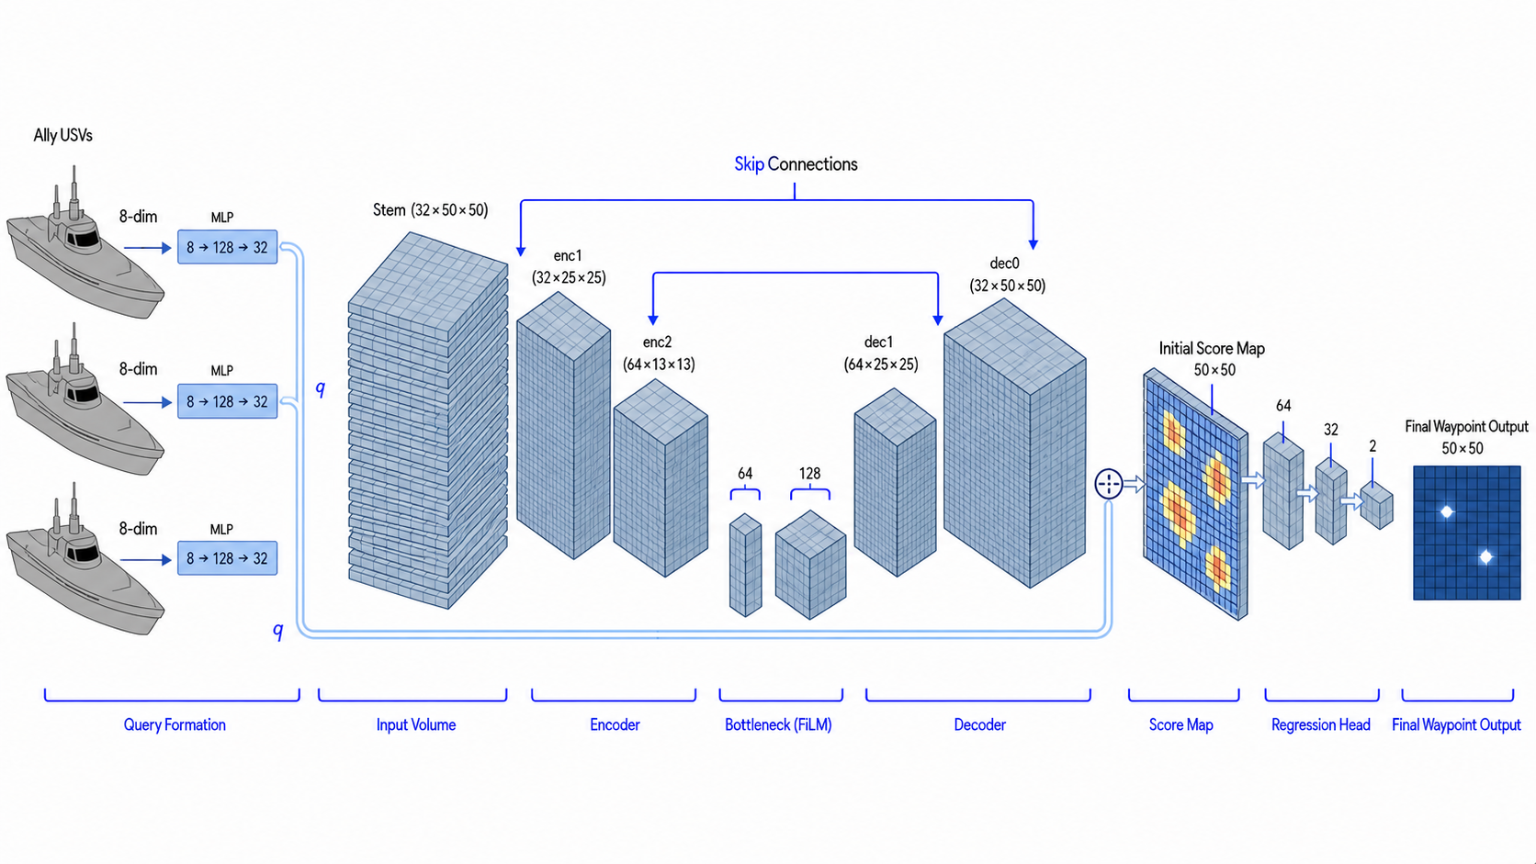
\includegraphics[width=0.66\textwidth]{fig8.png}
\caption{점수맵 정책의 구조: 질의·특징맵 내적과 칸 안 오프셋}
\label{fig:policy}
\end{figure*}

관측은 U-Net 구조~\citep{ronneberger2015unet}를 지나 입력과 같은 해상도의 특징 지도로
변환된다(Fig.~\ref{fig:policy}). 전역 평균 풀링으로 압축한 전황 벡터는
FiLM~\citep{perez2018film} 변조로 특징에 실려, 국소 합성곱이 옮기지 못하는 전황을 모든 위치에
전달한다.

각 방어정 $p$ 는 자신의 상태 벡터 $\mathbf{o}_p$ 로부터 MLP 로 질의 $\mathbf{q}_p$ 를 만들고,
아핀 사영 $\mathbf{W}_q$, $\mathbf{b}_q$ 를 거쳐 픽셀 $i$ 의 특징 $\mathbf{f}_i$ 와 내적하여
점수 $s_{p,i}$ 를 얻는다.
\begin{equation}
s_{p,i} = \frac{\langle \mathbf{W}_q \mathbf{q}_p + \mathbf{b}_q,\, \mathbf{f}_i \rangle}{\sqrt{d}}, \qquad d = 32
\label{eq:score}
\end{equation}
어텐션~\citep{vaswani2017attention}과 같은 형식의 점수로 격자 위의 원소를 지목하는 포인터
구조다~\citep{vinyals2015pointer}. 관측 텐서는 방어정을 묶어 결정마다 한 번의 순전파로 통과하며, 가중치는 모두가 공유하므로 모델 크기는 방어정 수에 불변이다. 합성곱 블록의 그룹
정규화~\citep{wu2018groupnorm}는 배치 통계를 쓰지 않아 묶음 크기와 무관하게 같은 연산이다.

\subsubsection{유효 마스크와 픽셀 지목}
\label{sec:validmask}

점수맵 전체가 후보가 되는 것은 아니다. 육지 픽셀 집합을 $\mathcal{L}_{\mathrm{land}}$, 모선에서
본 요격점 방위와 픽셀 방위의 차이를 $[0^\circ, 180^\circ]$ 로 접은 값을
$|\vartheta_i - \vartheta_p|_{\circ}$ 라 하면, 방어정 $p$ 의 유효 픽셀 집합 $\mathcal{V}_p$ 는
환상 요격 구역, 육지 밖, 요격점 반경, 무리 방위라는 네 조건의 교집합이다(설정값은
Table~\ref{tab:validmask_param}).
\begin{equation}
\begin{aligned}
\mathcal{V}_p = \big\{\, i :\; & r_{\min} \le \lVert \mathbf{x}_i - \mathbf{m} \rVert \le r_{\max},\;
  i \notin \mathcal{L}_{\mathrm{land}},\\
  & \lVert \mathbf{x}_i - \mathbf{I}_p \rVert \le r_{\mathrm{g}},\;
  |\vartheta_i - \vartheta_p|_{\circ} \le \vartheta_{\mathrm{g}} \,\big\}
\end{aligned}
\label{eq:validset}
\end{equation}
마스크는 로짓 단계에서 적용한다. 유효 집합 밖의 점수를 $-\infty$ 로 바꾼 마스크 점수
$\tilde{s}_{p,i}$ 를 소프트맥스에 넣어 픽셀 선택 확률을 얻는다.
\begin{equationsmall}
\tilde{s}_{p,i} = \begin{cases} s_{p,i}, & i \in \mathcal{V}_p \\ -\infty, & i \notin \mathcal{V}_p, \end{cases}
\quad
\pi_\theta(i \mid \mathbf{s}, p) = \frac{e^{\tilde{s}_{p,i}}}{\sum_{j \in \mathcal{V}_p} e^{\tilde{s}_{p,j}}}
\label{eq:masked_softmax}
\end{equationsmall}
안전·임무 제약이 손실 항이 아니라 행동 분포에 직접 부과되므로 위반은 애초에 표현 불가능하다.
학습된 체크포인트에서 격자 대부분은 갈 수 없는 자리로 남으며(Fig.~\ref{fig:validmask}), 연속
좌표 회귀에는 이 구조를 표현할 수단이 없다. 범주형 표본은 유효 영역을 벗어나지 않고 엔트로피가
유한하므로 \ref{sec:training}절의 그룹 후보들이 실제로 서로 다른 칸을 밟는다.

%============================================================ 유효 마스크·픽셀 지목 설정값 (국방발표 판)
%  §4.4.3 본문에 흩어져 있던 수치를 모은 표. 길이는 체계가 스케일 불변이므로 관측
%  픽셀 한 변 ell 기준의 비율로 적는다(기준 인스턴스의 m 값은 시나리오 표). 본문에는 기호와 논지만 남기고 값은 전부 여기에 둔다.
%  값 출처: boatattack_sim/env/config.py (cell_r_min/r_max, cnn_gate_r, cnn_gate_bear,
%           cnn_valid_min, cnn_nets, cnn_dup_r, net_max_len), 유효 비율은 학습 체크포인트 실측.
\begin{table}[htbp]
\centering
\caption{유효 마스크와 픽셀 지목의 설정값(\ref{sec:validmask}절)}
\label{tab:validmask_param}
\footnotesize
\resizebox{\ifdim\width>\linewidth\linewidth\else\width\fi}{!}{%
\begin{tabular}{llr}
\toprule
구분 & 기호 / 항목 & 값 \\
\midrule
\multirow{4}{*}{유효 픽셀 조건}
 & 요격 환형 안·바깥 반경 $r_{\min}$, $r_{\max}$ & $1.6\,\ell$ / $18\,\ell$ \\
 & 요격점 반경 조건 $r_{\mathrm{g}}$             & $12\,\ell$ \\
 & 무리 방위 조건 $\vartheta_{\mathrm{g}}$        & $60^\circ$ \\
 & 유효 픽셀 수 하한                              & $150$ 칸 \\
\midrule
\multirow{3}{*}{픽셀 지목}
 & 방어정 1척당 경유점 수 $K$                     & $2$ \\
 & 두 점 간격 하한 $r_{\mathrm{dup}}$             & $0.8\,\ell$ \\
 & 두 점 간격 상한                                & $1.5\,L_{\mathrm{net}}$ \\
\midrule
실측
 & 결정당 평균 유효 비율                          & $10.5\,\%$ \\
\bottomrule
\end{tabular}
}
\end{table}


\begin{figure*}[tbp]
\centering
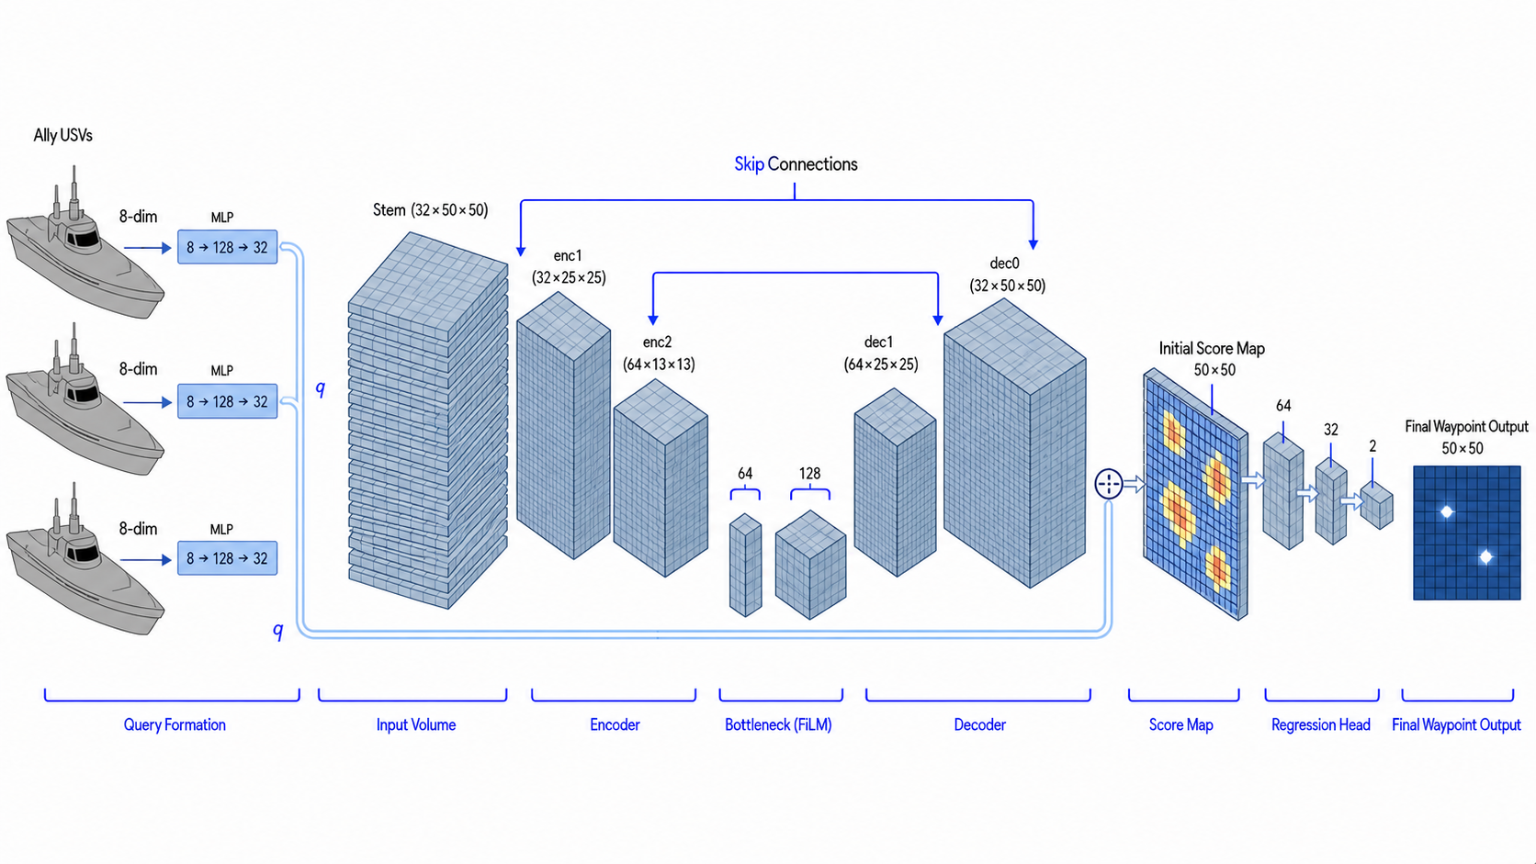
\includegraphics[width=\textwidth]{fig9.png}
\caption{유효 마스크와 픽셀 지목(학습된 체크포인트의 실제 출력)}
\label{fig:validmask}
\end{figure*}

각 방어정은 유효 영역 안에서 점수 상위 픽셀 $K$ 개를 순차적으로 고른다. 먼저 고른 픽셀의
특징을 질의에 더해 두 번째를 고르므로 두 점이 서로를 알고 뽑히며, 간격의 상·하한이 벽이 서지
않을 만큼 가까운 쌍과 그물 길이를 넘는 벽을 함께 배제한다. 칸 안 위치는 선택 픽셀의 특징으로부터
MLP 가 내는 평균과 학습되는 표준편차의 가우시안에서 표집해 칸의 절반 폭 $\ell/2$ 안에서
정하므로, 목표점 $\mathbf{t}_k$ 의 로그확률과 엔트로피는 범주형과 가우시안 두 분포의 합이다.

선택된 두 좌표를 잇는 선분이 그물벽 경로가 되며, 방어정은 가까운 점까지 이동한 뒤 다음
구간에서 그물을 전개한다. 그물이 없거나 배정되지 않은 방어정은 정지시킨다.

\subsection{가치망 없는 다중 에이전트 그룹 상대 최적화}
\label{sec:training}

\begin{figure}[!tbp]
\centering
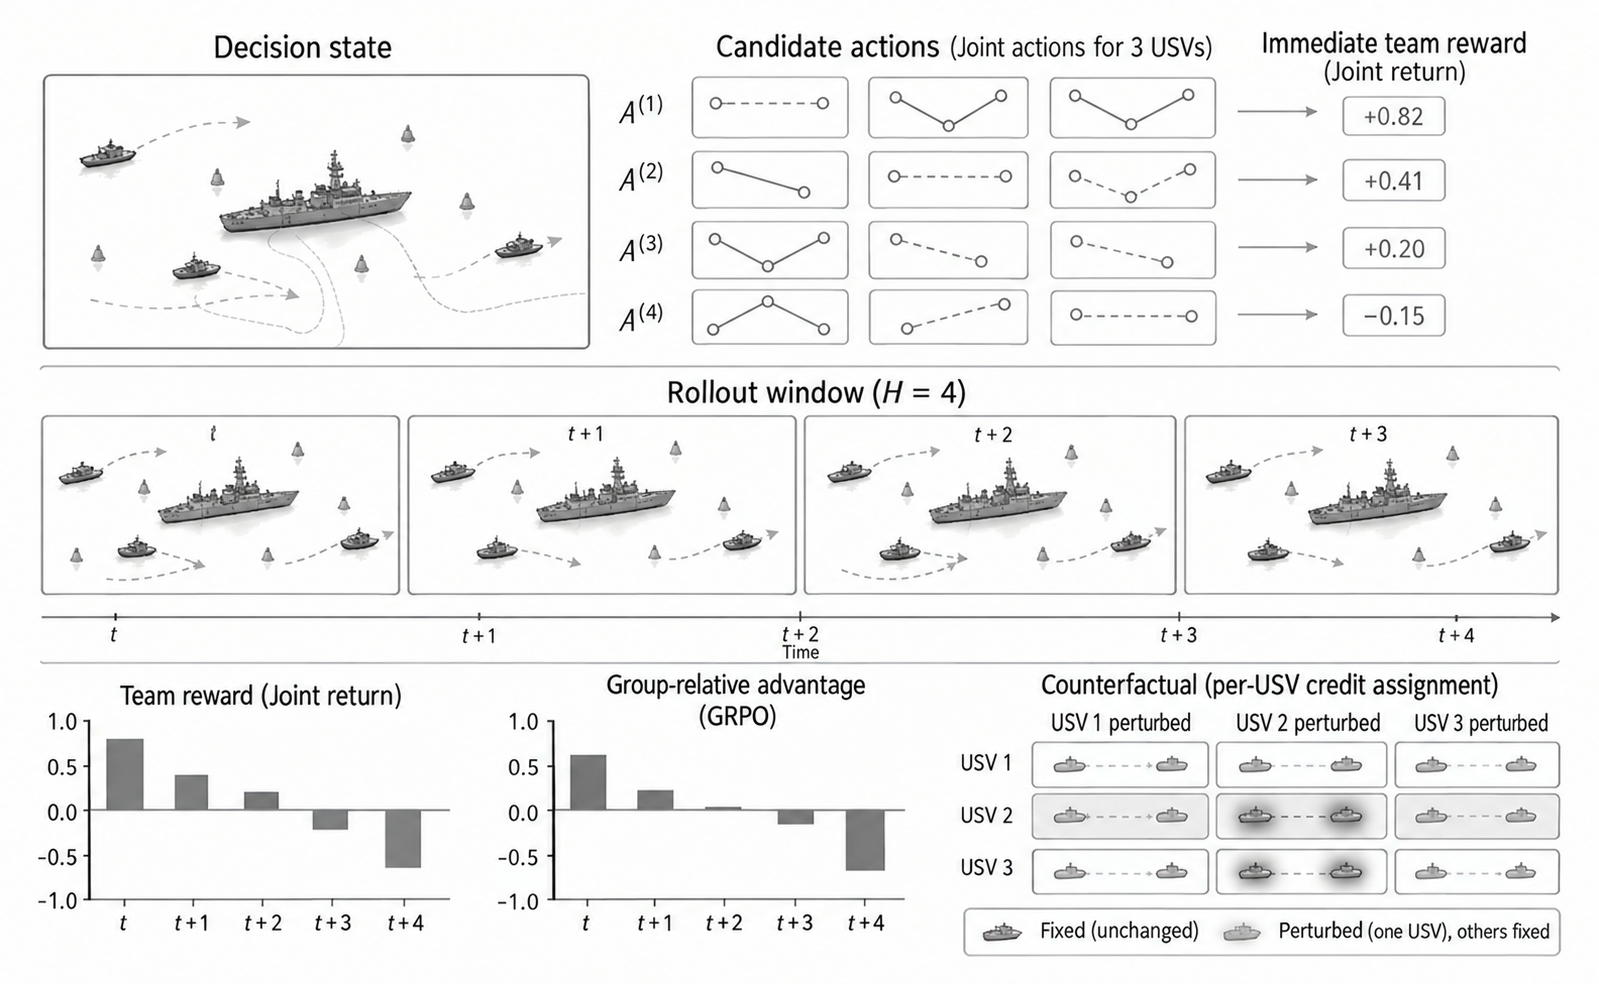
\includegraphics[width=\columnwidth]{fig11.png}
\caption{그룹 상대 최적화의 한 갱신(도식은 $G=4$, $H=4$)}
\label{fig:grpocredit}
\end{figure}

\subsubsection{그룹 상대 이득}

학습은 가치함수를 따로 두지 않는 그룹 상대 정책 최적화~\citep{shao2024deepseekmath}를 다중
방어정 상황에 맞게 변형하여 수행한다(Fig.~\ref{fig:grpocredit}). 매 결정 시점에서 정책으로부터
$G$개의 결합 행동 후보를 표집하되, 후보 가운데 하나($k=0$)는 휴리스틱(\ref{sec:heuristic}절)이
내는 행동으로 고정하여 기준선으로 삼는다. 각 후보를 시뮬레이터에서 공통 구간
$H = 180\,\mathrm{step}$ 만큼 실제로 진행시켜 창 보상 $R_k$ 를 얻은 뒤(\ref{sec:reward}절),
휴리스틱 후보의 보상 $R_0$ 를 기준으로 상대 비교하여 이득 $A_k$ 를 산정한다. 그룹 표준편차로 나누되 $\epsilon$ 을 더해 0 나눗셈을 막는다.
\begin{equation}
A_k = \frac{R_k - R_0}{\mathrm{std}(\{R_j\}_{j=0}^{G-1}) + \epsilon}
\label{eq:adv}
\end{equation}
휴리스틱을 넘어서는 후보만 양의 이득을 받고, 그룹 표준편차로 나누므로 이득은 크기가 없는
순위 정보만 남는다. 어떤 선택이 더 나았는지를 실제 결과로 직접 비교하므로 가치망과 그 추정
편향·학습 불안정이 없다.

한 갱신은 $N$개의 병렬 전장(월드)에서 동시에 수행된다. 후보 보상이 모두 같은 월드는 이득이
정의되지 않으므로 유효 월드 마스크 $w_n$ 으로 갱신에서 제외한다. 월드 $n$ 의 상태를
$\mathbf{s}_n$, 후보 $k$ 의 이득을 $A_{n,k}$, 그 후보에서 방어정 $p$ 의 행동을
$a^{(k)}_{n,p}$ 라 하면, 정책경사 손실은 유효 월드의 모든 후보·모든 방어정에 대해 이득으로
가중한 로그확률의 음수이다.
\begin{equationfn}
\mathcal{L}_{\mathrm{PG}}(\theta) = -\frac{\sum_{n} w_n \sum_{k=0}^{G-1} A_{n,k} \sum_{p=1}^{P} \log \pi_\theta\big(a^{(k)}_{n,p} \mid \mathbf{s}_n\big)}{G \sum_n w_n}
\label{eq:lpg}
\end{equationfn}
여기에 엔트로피 정칙화를 더한 총손실을 최소화하며, 기울기 노름을 클립한 뒤 갱신한다.

\label{sec:bc}
\label{sec:schedule}
그룹 상대 이득은 후보들이 갈릴 때만 신호를 주므로, 학습에 앞서 휴리스틱
행동(\ref{sec:heuristic}절)을 목표로 짧은 행동 복제로 정책을 부팅한다. 목표는 원-핫이 아니라
휴리스틱 픽셀을 중심으로 한 폭 좁은 가우시안을 유효 픽셀 위에서 정규화한 가중이다. 옵티마이저는 Adam 이며, 학습률은 $10^{-4}$ 에서 그 $5\,\%$ 까지
단일 주기 코사인 어닐링~\citep{loshchilov2017sgdr}으로, 엔트로피 계수는 $0.01$ 에서 그
$10\,\%$ 까지 선형으로, 총 800 업데이트의 같은 예산 축 위에서 함께 줄인다. 나머지 상수는
Table~\ref{tab:hparams}에 모았다.

\subsubsection{보상 설계}
\label{sec:reward}

한 후보의 창 보상은 결정 시점부터 $H$\,step 동안 일어난 일을 하나의 스칼라로 합산한 팀 공유
보상이며, 이벤트 항 $R_\mathrm{event}$, 창의 시작·끝 상태에서 잰 퍼텐셜 $\Phi$ 의
할인($\gamma$) 차분, 조밀 항 $R_\mathrm{dense}$ 로 구성된다. 세 항의 계수는
Table~\ref{tab:reward_coef}에 모았다.
\begin{equation}
R = R_\mathrm{event} + \big[\gamma\,\Phi(\mathbf{s}_{t+H}) - \Phi(\mathbf{s}_t)\big] + R_\mathrm{dense}
\label{eq:reward}
\end{equation}

\begin{table}[tp]
\centering
\caption{보상 계수}
\label{tab:reward_coef}
\footnotesize
\renewcommand{\arraystretch}{1.15}
\begin{tabular}{@{}llr@{\hspace{2mm}}l@{}}
\toprule
항 & 기호 & 값 & 의미 \\
\midrule
\multirow{6}{*}{이벤트}
 & $r_{\mathrm{cap}}$  & $+13.5$ & 포획 1건 \\
 & $r_{\mathrm{brc}}$  & $-8.0$  & 돌파 1건 \\
 & $r_{\mathrm{col}}$  & $-30$   & 충돌·육지 충돌 1건 \\
 & $r_{\mathrm{tng}}$  & $-13$   & 그물 접촉 1건 \\
 & $r_{\mathrm{wipe}}$ & $+8$    & 창 안 종료 시 전멸 \\
 & $r_{\mathrm{surv}}$ & $-5$    & 창 안 종료 시 잔존 적 1척당 \\
\midrule
\multirow{3}{*}{퍼텐셜}
 & $w_{\mathrm{threat}}$ & $3.0$  & 모선 근접도 합의 가중 \\
 & $R_w$                 & 25\,$\ell$ & 근접도 정규화(교전 해역 반폭) \\
 & $\gamma$              & $0.99$ & 할인 \\
\midrule
\multirow{10}{*}{조밀}
 & $w_{\mathrm{path}}$ & $0.5$  & 이동거리 비용 \\
 & $w_{\mathrm{net}}$  & $0.3$  & 그물 소모 비용 \\
 & $w_{\mathrm{turn}}$ & $0.3$  & 선회량 비용 \\
 & $w_{\mathrm{cons}}$ & $0.3$  & 목표점 일관성 비용 \\
 & $w_{\mathrm{prox}}$ & $0.75$ & 모선·타 방어정 근접 비용 \\
 & $w_{\mathrm{cov}}$  & $0.1$  & 커버리지 보너스 \\
 & $w_{\mathrm{ray}}$  & $1.6$  & 배율판 보너스 \\
 & $R_{\mathrm{m}}$      & 3.2\,$\ell$ & 모선 안전 반경 \\
 & $\varrho_{\mathrm{m}}$ & 2.0\,$\ell$ & 모선 근접 영향 반경 \\
 & $\varrho_{\mathrm{a}}$ & 2.4\,$\ell$ & 타 방어정 근접 영향 반경 \\
\bottomrule
\end{tabular}
\end{table}

이벤트 항은 창 안의 포획·돌파·충돌·그물 접촉 건수에 고정 가중을 곱한 합이며, 창 안에서
에피소드가 끝나면 전멸 보너스와 잔존 적 1척당 벌점을 더한다. 퍼텐셜 $\Phi$ 는 생존 적선의
모선 근접도 합에 가중을 곱해 부호를 바꾼 것이라 적이 포획되거나 멀어지면 오르며, 할인 차분 형태로 주어지므로 최적 정책을
보존한다~\citep{ng1999shaping}. 조밀 항은 기동 품질에 대한 비용·보너스의 합으로, 이동거리·소모
그물 수·선회량·직전 결정 대비 목표점 이동과 모선·타 방어정 근접도를 벌하고, 설치된 그물이 적의
접근로를 막는 비율(커버리지)을 보상한다. 포획은 평가 창의 $46.8\,\%$ 에서만 일어나므로,
나머지 창에서는 퍼텐셜·커버리지 항이 후보 순위를 가르는 주된 신호다.

\subsection{언어모델 기반 전략 계층}
\label{sec:commander}
\label{sec:schema}

전략 계층의 입력은 전장 상태·임무 목표·교전 규칙·자산 상태이고, 출력은 무리별 배정과 대기(HOLD)이며, 그 배정이 기동 계층으로 전달되어 각
방어정의 그물벽 위치 결정을 조건짓는다.

언어모델에는 좌표 원시 데이터 대신 기하량이 미리 계산된 전장 상태를 텍스트로 전달한다.
각 적 무리의 요격점까지의 이동거리와 선회량, 모선 기준 방위, 설치된 그물에 의한 접근로 차단
여부가 포함된다. 출력은 자유 문장이 아니라 다음 자료형이 정하는 JSON
형식으로 강제한다~\citep{openai2026function}. 자유 문장은 파싱에 실패하면 그 주기의 배정을
통째로 잃지만, 이 형식은 디코딩 단계에서 문법으로 작용해 어긋난 토큰 자체를 막는다.

\begin{quote}\ttfamily\scriptsize\setlength{\parindent}{0pt}
CommanderPlan \{\\
\hspace*{1.2em} rationale: str\\
\hspace*{1.2em} deployments: List[\{\\
\hspace*{3.0em} cluster\_id: int,\\
\hspace*{3.0em} ally\_ids: List[int] \}]\\
\hspace*{1.2em} hold\_ships: List[int]\\
\}
\end{quote}

언어모델이 정하는 것은 어느 배가 어느 무리를 맡는가뿐이고 나머지는 대기다. 그물 전개
여부·벽의 방위·교전 반경과 요격점 기하는 기동 계층이 정하며, 배정은 코드가 보정하지 않고
그대로 쓰인다.

한 무리에 두 척 이상이 배정되면 \ref{sec:heuristic}절의 잉여 배정과 같은 반경·방위 분리가
작동하되, 요격점이 요격 구역을 벗어나 유효 마스크가 붕괴하지 않도록 반경을 구역 안으로 자른다.
배정이 바뀌면 요격점과 함께 기동 계층의 유효 마스크(\ref{sec:validmask}절)도 바뀌므로, 배정은
기동의 선행 조건이다.

%============================================================ 5. 실험 설계 (압축판)
%  모델명은 이 절에서 한 번만 밝히고, 이후 본문은 능력 수준(소형·중형·상위)으로 지칭한다.
%  능력 임계 주장이 특정 모델 세대나 서빙 방식에 묶이지 않게 하려는 의도다.
%  발표판은 절을 둘로만 둔다: (1) 환경과 학습 실행, (2) 조건·판정·계측.
\section{실험 설계}
\label{sec:experiment}

두 계층의 기여를 분리하기 위해 배정 축과 기동 축을 각각 이분한 $2\times2$ 조건 행렬을 두고,
시드 대응 차이로 판정한다.

\subsection{환경과 학습 실행}
\label{sec:env}
\label{sec:protocol}

교전 설정값은 Table~\ref{tab:scenario}, 지표는 Table~\ref{tab:metrics}를 따르고, 지휘관
재계획은 매 결정마다 수행한다. 지휘관으로는 능력 수준이 다른 소형 Qwen2.5 7B, 중형
Qwen2.5 14B, 상위 Gemini 3.5 Flash-Lite 를 온도 0, 같은 프롬프트, 같은 구조적
출력(\ref{sec:schema}절)으로 쓰며, 이하 본문은 이들을 능력 수준으로 지칭한다.

시뮬레이터의 물리·판정 모델과 단순화는 Table~\ref{tab:simfidelity}에 모았다. 실선
동역학~\citep{fossen2011marine} 대신 쓴 질점 운동학, 규칙 기반의 적, 잡음 없는 완전 관측은 모두
방어에 유리하므로 포획률은 상한이며, 네 조건이 같은 가정을 공유하므로 조건 간 상대 비교로만
판정한다.

\inputshortcap{시뮬레이터의 물리·판정 모델과 단순화}{tables/tab_simfidelity}

%  ★ 언리얼 엔진 검증 환경의 언급과 도판(fig_ue_env)은 필수다 --- 분량을 줄일 때도
%    지우지 말 것. 모델 성능을 이 환경에서 검증한다.
학습은 질점 운동학 시뮬레이터에서 수행하고, 학습된 정책의 성능은 선체 거동과 충돌을 물리
엔진으로 다루는 언리얼 엔진 환경(Fig.~\ref{fig:ue_env})에서 검증한다. \ref{sec:results}절의
통계 비교는 같은 시드 집합을 조건마다 되풀이 수집해야 하므로 질점 시뮬레이터에서 수행하였다.

\begin{figure*}[tp]
\centering
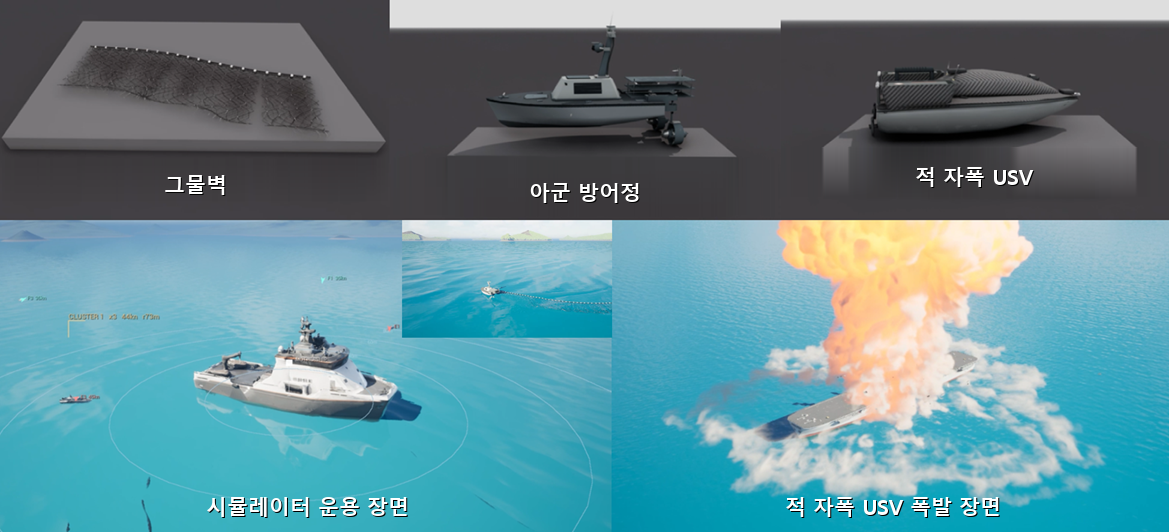
\includegraphics[width=0.92\textwidth]{fig_ue_env.png}
\caption{언리얼 엔진 기반 시뮬레이터에서의 정성 검증}
\label{fig:ue_env}
\end{figure*}


학습은 한 해안선 형상에 과적합하지 않도록 실해역 6곳(Fig.~\ref{fig:sites})을 에피소드마다
돌려가며 진행하고, 평가는 그중 통영 매물도 서측에서 한다. 학습 설정은
Table~\ref{tab:hparams}에 모았으며, 주기적 greedy 평가의 최고점 가중치를 채택하였다.

\begin{figure}[!tbp]
\centering
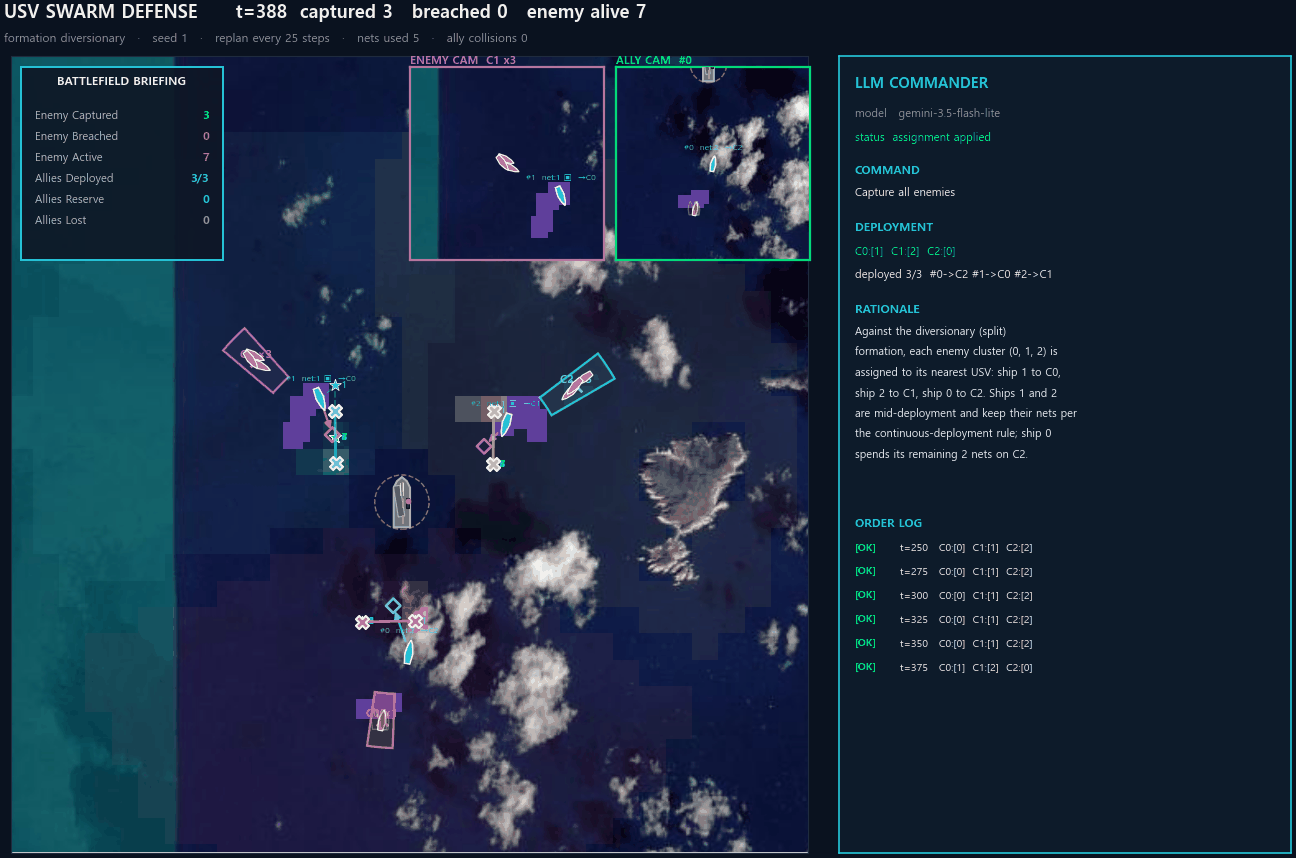
\includegraphics[width=0.88\columnwidth]{fig14.png}
\caption{학습 해역 6곳(별표 모선, 파선 원 요격 구역)}
\label{fig:sites}
\end{figure}

\inputshortcap{기동 정책 학습 설정}{tables/tab_hparams}

\subsection{조건, 판정 기준, 계측}
\label{sec:paired}
\label{sec:stats}

\begin{table}[!htb]
\centering
\caption{$2\times2$ 조건 행렬(조건 사이 차이는 두 스위치뿐)}
\label{tab:conditions}
\footnotesize
\setlength{\tabcolsep}{3pt}
\begin{tabular}{llp{0.34\linewidth}}
\toprule
조건 & 배정 $\times$ 기동 & 무엇을 측정하는가 \\
\midrule
\texttt{heur\_heur} & 휴리스틱 $\times$ 휴리스틱 & 기준선(baseline) \\
\texttt{heur\_unet} & 휴리스틱 $\times$ U-Net    & 기동 계층의 순수 기여(LLM 미사용) \\
\texttt{llm\_heur}  & LLM $\times$ 휴리스틱      & 전략 계층의 순수 기여 \\
\texttt{llm\_unet}  & LLM $\times$ U-Net         & 제안 체계(상호작용 포함) \\
\bottomrule
\end{tabular}
\end{table}

휴리스틱 배정과 기동은 \ref{sec:heuristic}절의 기준 방법이며 학습 정책과 같은 행동공간을
거치므로 네 조건은 직접 비교 가능하다(Table~\ref{tab:conditions}). 전략 계층에 세 모델을 두고
모든 조건이 같은 시드 집합과 세 포메이션을 공유하도록 하여 720 에피소드를 수집하였다.

갱신 규칙 자체를 가르기 위해, 같은 액터·관측·행동공간·보상·행동복제 초기화 위에서 갱신 규칙만
MAPPO~\citep{yu2022mappo}로 바꾼 정책을 시드 3개로 학습하고, 같은 step 예산과 같은 프로토콜로
평가한다(\ref{sec:res_algo}절).

조건과 기준선의 시드 $k$ 지표값을 $x_k$, $y_k$, 시드 수를 $n_{\mathrm{s}}$, 대응 차이 $d_k$ 의
표준편차를 $s_d$ 라 하면 차이의 평균과 효과크기는
\begin{equation}
d_k = x_k - y_k, \qquad
\bar{d} = \frac{1}{n_{\mathrm{s}}}\sum_{k} d_k, \qquad
\dz = \frac{\bar{d}}{s_d}
\label{eq:paired}
\end{equation}
이며, $\bar{d}$ 의 95\,\% 신뢰구간은 편향 보정·가속(bias-corrected and accelerated, BCa)
부트스트랩~\citep{efron1993bootstrap, diciccio1996bca}($B = 9999$)으로 구한다. 구간이 0을
포함하면 기준선과 다르다고 말하지 않으며, 지표 10개의 다중비교에는 Bonferroni 보정
구간(99.5\,\%)을 병기한다. 두 계층의 상호작용은 배정 축(H 휴리스틱, L 언어모델)과 기동
축(H 휴리스틱, U U-Net)으로 쓴 조건 $(a, m)$ 의 지표값 $x_k^{am}$ 에서
\begin{equation}
\mathrm{Int}_k = \big(x_k^{\mathrm{LU}} - x_k^{\mathrm{LH}}\big)
               - \big(x_k^{\mathrm{HU}} - x_k^{\mathrm{HH}}\big)
\label{eq:interaction}
\end{equation}
의 평균과 신뢰구간을 식~\eqref{eq:paired}와 같은 절차로 구해 판정한다($>0$ 상승,
$\approx 0$ 가산, $<0$ 상쇄).

포획률은 체계 전체의 지표라 지휘관 계층의 기여를 가리므로, 계획 산출 시점에 확인 가능한 양을
따로 계측한다: 응답 지연, 폴백률(언어모델 실패로 휴리스틱이 대체한 비율), 커버리지(활성 무리
중 배정된 비율), churn(재계획 간 담당을 바꾼 방어정 비율), 교차 배정(방어정--담당 무리 선분이
서로 교차하는 쌍의 수). 뒤의 세 양은 재계획에 걸쳐 평균한다.

%============================================================ 6. 결과 (압축판)
%  지휘관(LLM) 계층은 본 연구의 기여가 아니라 사용한 구성요소이므로, §6.2 는 표 두 개로
%  줄이고 도판을 두지 않는다. 도판은 기동 계층·체계 전체의 주장에만 쓴다.
\section{결과}
\label{sec:results}

\subsection{기동 계층의 기여}
\label{sec:res_g1}

\subsubsection{휴리스틱 대 점수맵 정책}
\label{sec:res_maneuver}

언어모델 없이 \ref{sec:heuristic}절의 기하 휴리스틱과 \ref{sec:policy}절의 점수맵 정책만
비교한다. 배정은 둘 다 휴리스틱이므로 차이는 기동 방식뿐이다(Table~\ref{tab:maneuver}). 3개
포메이션 통합 기준으로 포획률은 $0.844 \to 0.886$($\dz = 0.37$)으로 $95\,\%$ 수준에서
유의하나, 다중비교 보정을 걸면 구간이 0을 포함한다(\ref{sec:stats}절). 기동 계층이 바꾸는 것은 포획률이 아니라 자원과
기동이다.

\inputshortcap{기동 계층(U-Net 점수맵 + GRPO)의 단독 기여}{tables/tab_maneuver}

\begin{figure}[!tbp]
\centering
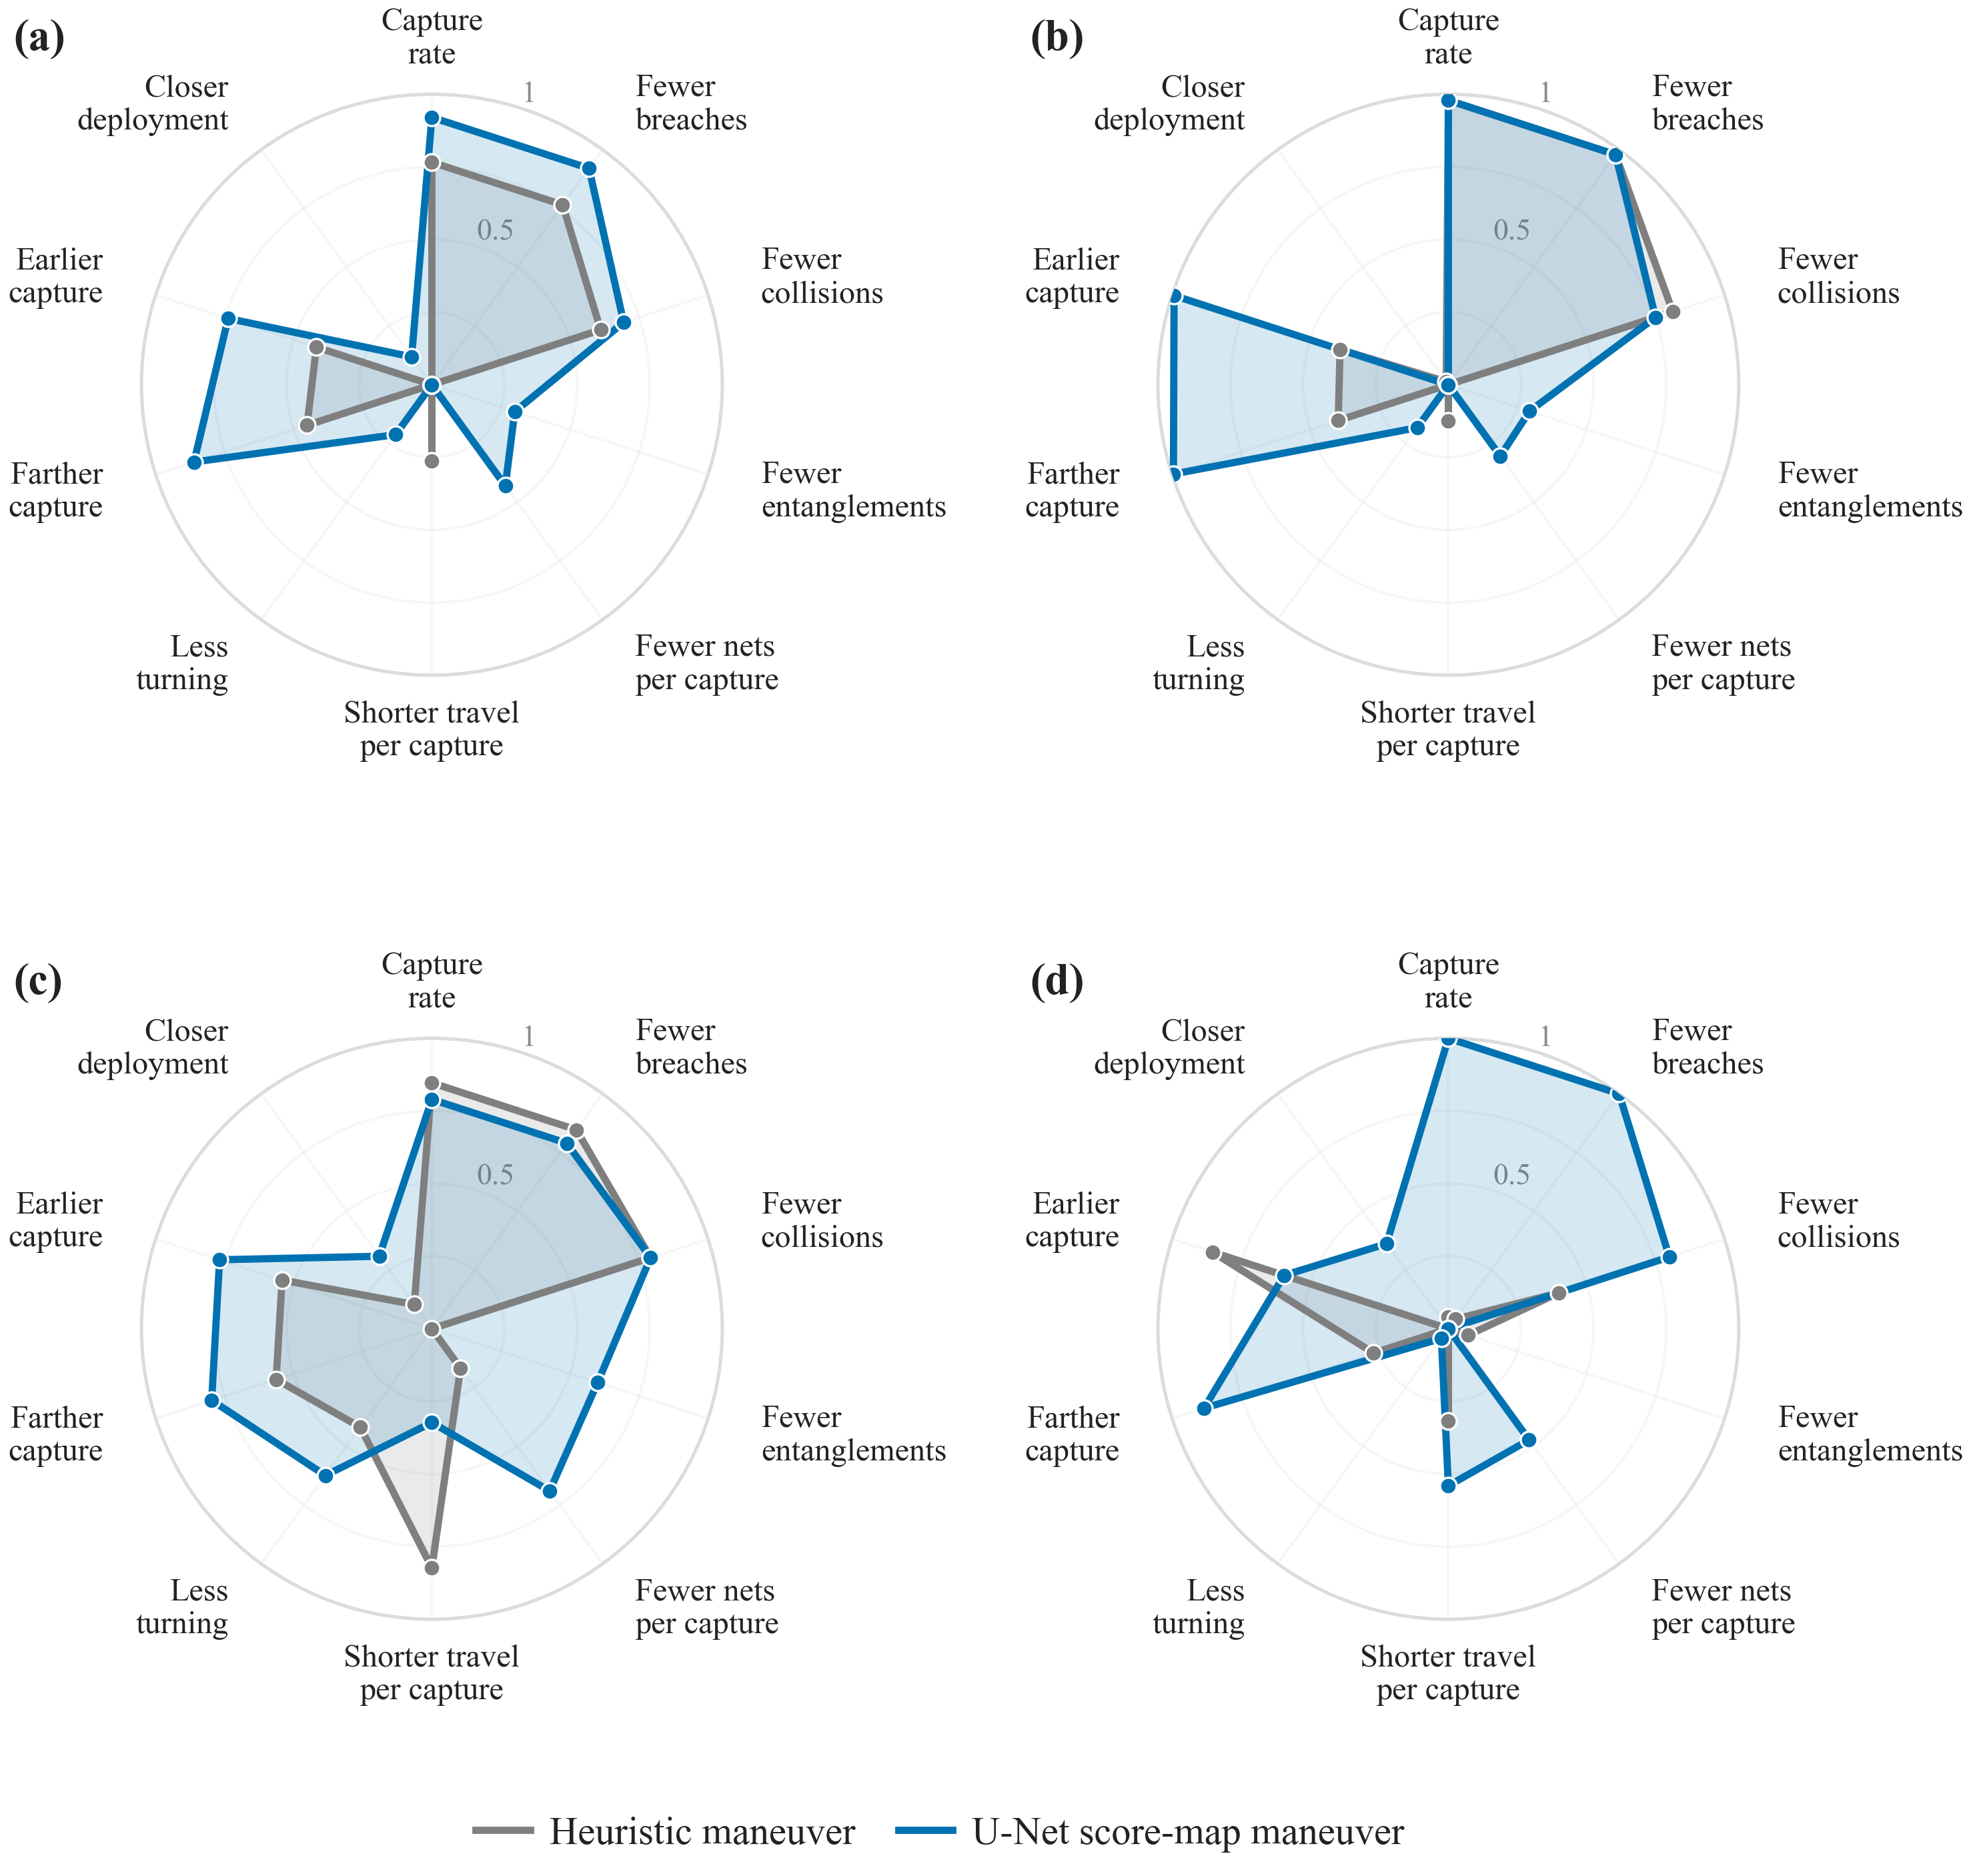
\includegraphics[width=\columnwidth]{fig15.png}
\caption{지표 프로파일: a 전체, b 집중, c 양동, d 파상}
\label{fig:radar_maneuver}
\end{figure}

같은 비교를 10개 지표 전부로 넓히면(Fig.~\ref{fig:radar_maneuver}, 각 축은 8개 조건의
범위로 0--1 정규화) U-Net 은 포획당 이동거리 축에서만 안쪽이다. 자리를 골라
그물벽을 놓는 대신 더 멀리 움직이기 때문이다. 충돌률·전개 시 적 거리 축은 겹치고, 나머지 일곱 축에서
바깥에 있다.

포메이션별로 보면 기여가 고르지 않다. 파상에서 $+0.157$($\dz = 0.48$)로 가장 크고, 집중에서는
$0.000$, 양동에서는 $-0.033$ 으로 오히려 소폭 낮다(유의하지 않아 악화로 읽지는 않는다).
\ref{sec:scenario}절의 포메이션 구조가 이 대비를 설명한다. 파상에서는 앞 단을 막은 그물벽의
위치가 뒤 단의 차단을 좌우하므로 해면 전체를 평가하는 점수맵이 직접 효과를 내고, 양동에서는 무리 수와 방어정 수가 같아 결정적인 것이 배정이라 배정이
어긋나면 기동이 보정하지 못한다. 집중은 휴리스틱만으로 포획률 0.997에 도달해 개선
여지가 남지 않는 구간이다(\ref{sec:res_ceiling}절).

\subsubsection{갱신 규칙: 그룹 상대 최적화 대 MAPPO}
\label{sec:res_algo}

점수맵 정책의 이득이 픽셀 지목이라는 표현에서 오는지 가치망 없는 갱신 규칙에서 오는지를
가르기 위해, 같은 액터·행동공간·보상·예산 위에서 갱신 규칙만 MAPPO 로 바꾼 정책 세 개를 같은
프로토콜로 평가하였다(Table~\ref{tab:algo}).

\inputshortcap{같은 픽셀 행동공간 위의 학습 알고리즘 비교}{tables/tab_algo}

포획률은 갈리지 않는다. MAPPO $0.859$ 와 GRPO $0.886$ 의 차이는 유의하지 않고, 포메이션별
방향도 파상 개선·양동 저하로 같다. 갈리는 것은 자원과 조기 제압이다. MAPPO 의 프로파일은
포획률·돌파 축을 빼면 휴리스틱 위에 그대로 겹치는 반면, GRPO 는 포획당 그물을
$0.737 \to 0.568$ 로 줄이고($\dz = -1.19$), 포획 이격거리를 $154\unit{m}$ 늘리며($\dz = +1.21$),
평균 포획 시각과 전개 시 적 거리도 앞당긴다. 네 지표 모두 다중비교 보정에서도 유의하다.
MAPPO 가 이기는 축은 포획당 이동거리 하나다.

같은 표현을 공유하는 한 갱신 규칙은 포획률을 가르지 못하고 그물 절약과 조기 제압만
좌우한다. 휴리스틱 후보를 기준으로 삼는 그룹 상대 이득(\ref{sec:training}절)은 휴리스틱을
넘어서는 선택에만 양의 이득을 주어 그 자원 사용 패턴에서 벗어나게 하는 반면, 팀 가치로
학습하는 MAPPO 는 어느 배가 그물을 아꼈는지를 개별 배에 귀속시킬 신호가 약하다.

\subsection{지휘관 계층의 기여}
\label{sec:res_g2}
\label{sec:res_main}
\label{sec:res_threshold}
\label{sec:res_ceiling}
\label{sec:res_mechanism}
\label{sec:res_latency}

지휘관 계층은 가져다 쓴 구성요소이므로 모델 사이의 순위가 아니라 배치에 필요한 것만 본다.
기동 계층을 휴리스틱으로 고정해 지휘관 축만 분리하면 포획률은 모델 능력을 따라 단조로 오르되,
능력이 낮은 쪽은 휴리스틱 배정 기준선에 미치지 못한다(Table~\ref{tab:main},
Fig.~\ref{fig:condbars}). 개선 폭은 포메이션에 따라 갈려, 휴리스틱만으로 이미 포화한 집중에는
남는 여지가 없고 여유가 없는 양동과 파상에서 크다. 성능을 가르는 것은 배정
커버리지가 아니다(Table~\ref{tab:planquality}). 가장 낮은 성능의 모델이 커버리지는 가장
높았으므로 막아야 할 무리를 빠뜨려서 지는 것이 아니며, 성능과 맞물린 양은 재계획 간 담당
변경(churn)과 경로 교차였다. 재계획마다 방어정의 약 3분의 1이 담당을 바꾸면 그때까지 전개하던
그물벽과 이동이 회수되지 않고, 두 방어정의 진로가 서로를 가로지르는 배정은 충돌 위험을 높인다.
지연도 배치 조건을 가른다. 중형 모델은 응답이 간헐적으로 결정 주기를 넘겨 동기 구조라면 그동안
제어 루프가 멈추므로, \ref{sec:arch}절은 전략 계층만 비동기로 떼어 둔다.

\inputshortcap{조건별 포획률(평균, 95\,\% CI, baseline 대비 차이)}{tables/tab_main}

\begin{figure}[!tbp]
\centering
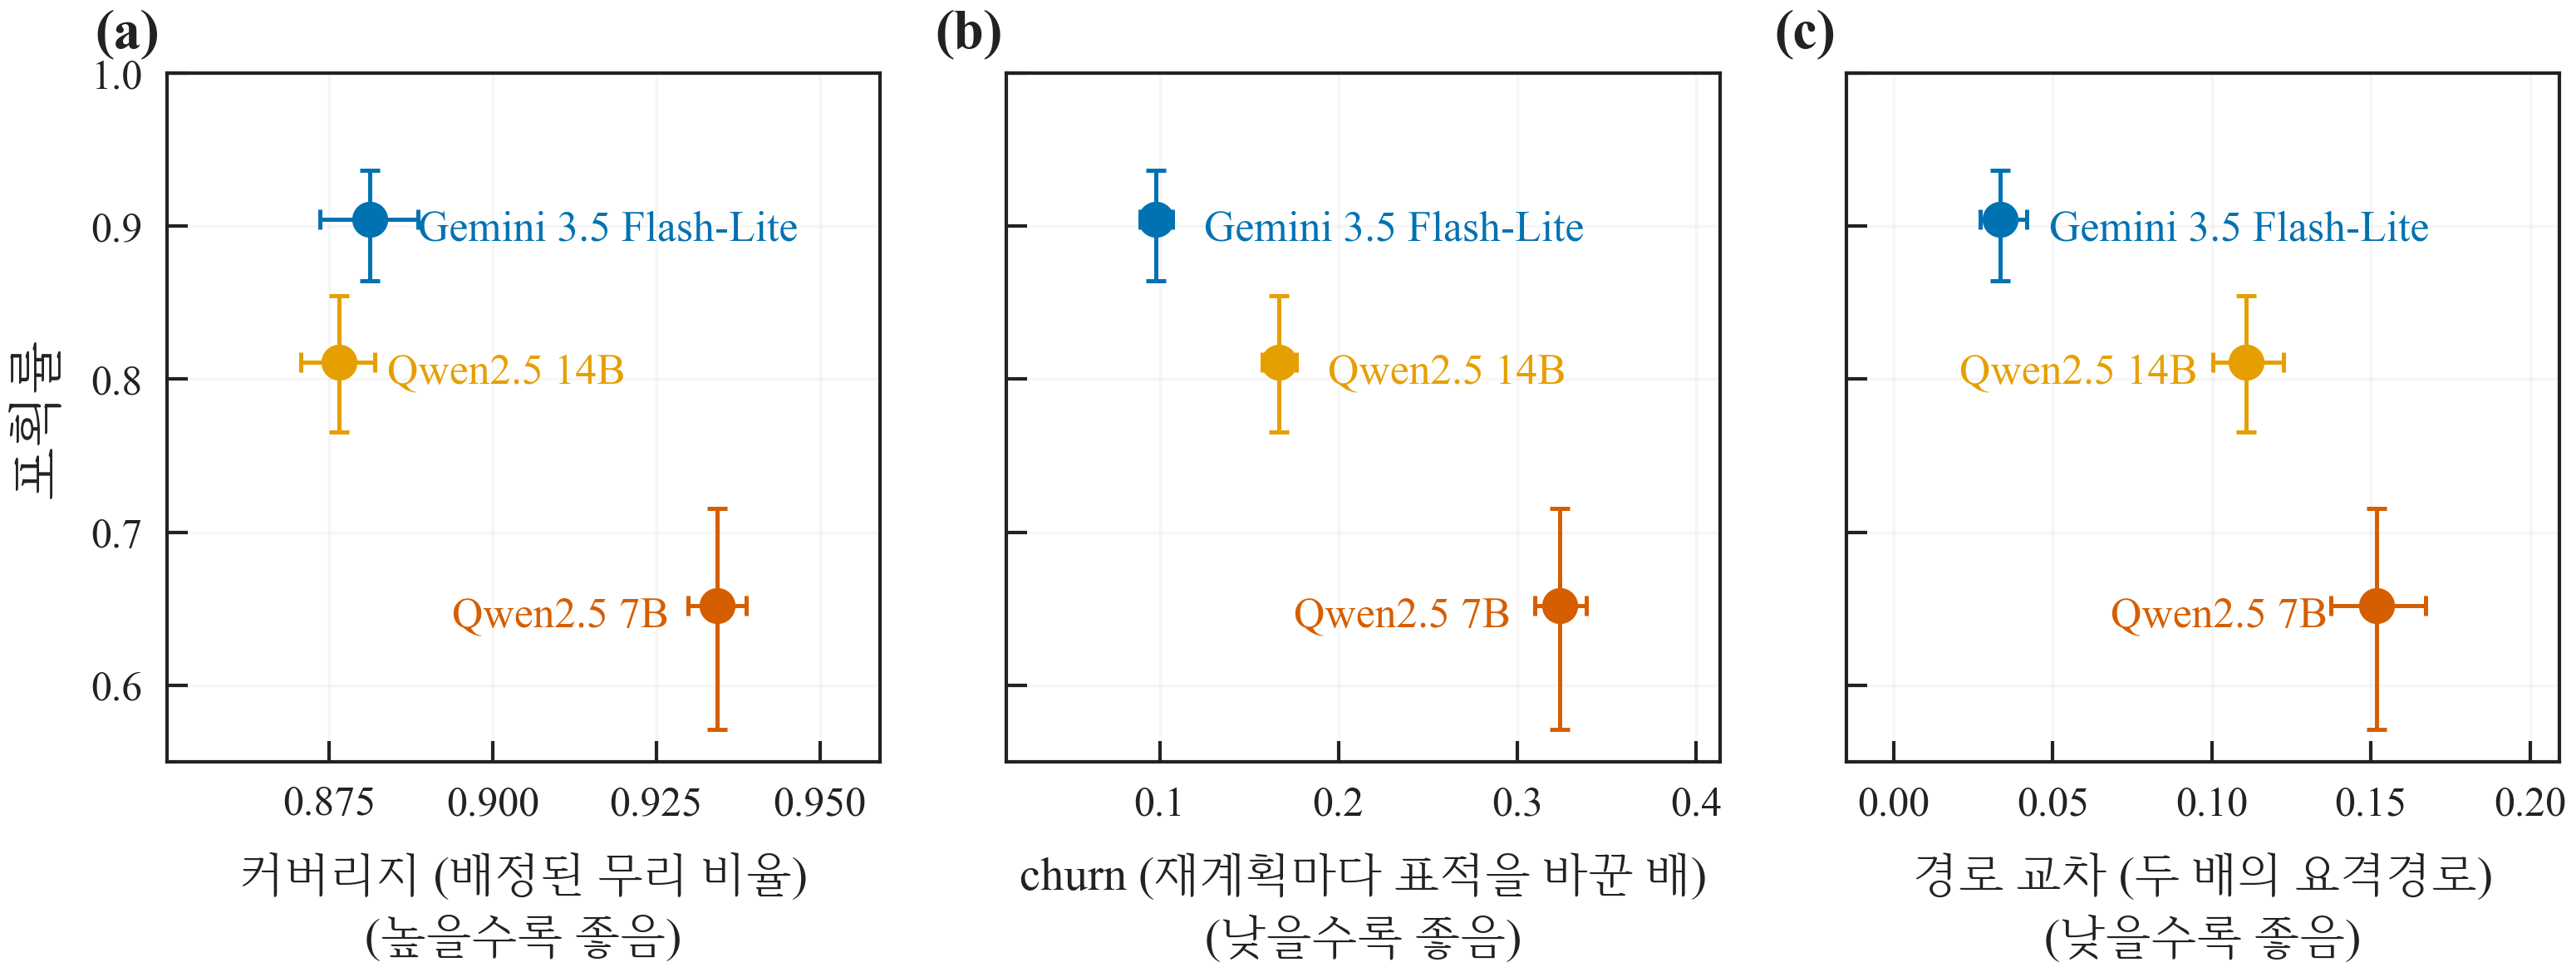
\includegraphics[width=\columnwidth]{fig18.png}
\caption{포메이션별·조건별 포획률(오차막대 95\,\% CI)}
\label{fig:condbars}
\end{figure}

\inputshortcap{지휘관 계획 품질과 성능}{tables/tab_planquality}

\subsection{제안 체계 전체}
\label{sec:res_g3}

\subsubsection{두 계층의 상호작용}
\label{sec:res_interaction}

식~\eqref{eq:interaction}의 상호작용을 10개 지표 전부에 대해 계산하였다(Table~\ref{tab:interaction}).

\inputshortcap{$2\times2$ 상호작용 분해(Gemini 지휘관)}{tables/tab_interaction}

10개 지표 중 9개에서 상호작용이 유의하지 않고, 다중비교 보정 후에도 그대로 9개다. 두 계층의 기여는 상승이 아니라 가산적이다. 예외인 평균 포획 시각은
유의한 상쇄인데, 두 계층 모두 제압을 앞당기는 쪽으로 작용하므로 같은 포획을 두 번 앞당길
수는 없는 수확체감이다. 가산성이 두 계층을 따로 써도 된다는 뜻은 아니다. 양동에서는 기동
계층 단독($-0.033$)도 전략 계층 단독($+0.070$)도 유의하지 않은데 결합은 $+0.090$ 으로
유의해진다. 무리 수와 방어정 수가 같아 배정과 기동이 둘 다 맞아야 막히기 때문이다.

\subsubsection{전 지표 효과크기}
\label{sec:res_effectsize}

제안 체계와 기준선의 차이를 10개 지표에 걸쳐 효과크기로 잰다(Table~\ref{tab:effectsize},
Fig.~\ref{fig:forest}).

\inputshortcap{전 지표 효과크기($|\dz|$ 내림차순)}{tables/tab_effectsize}

\begin{figure}[!tbp]
\centering
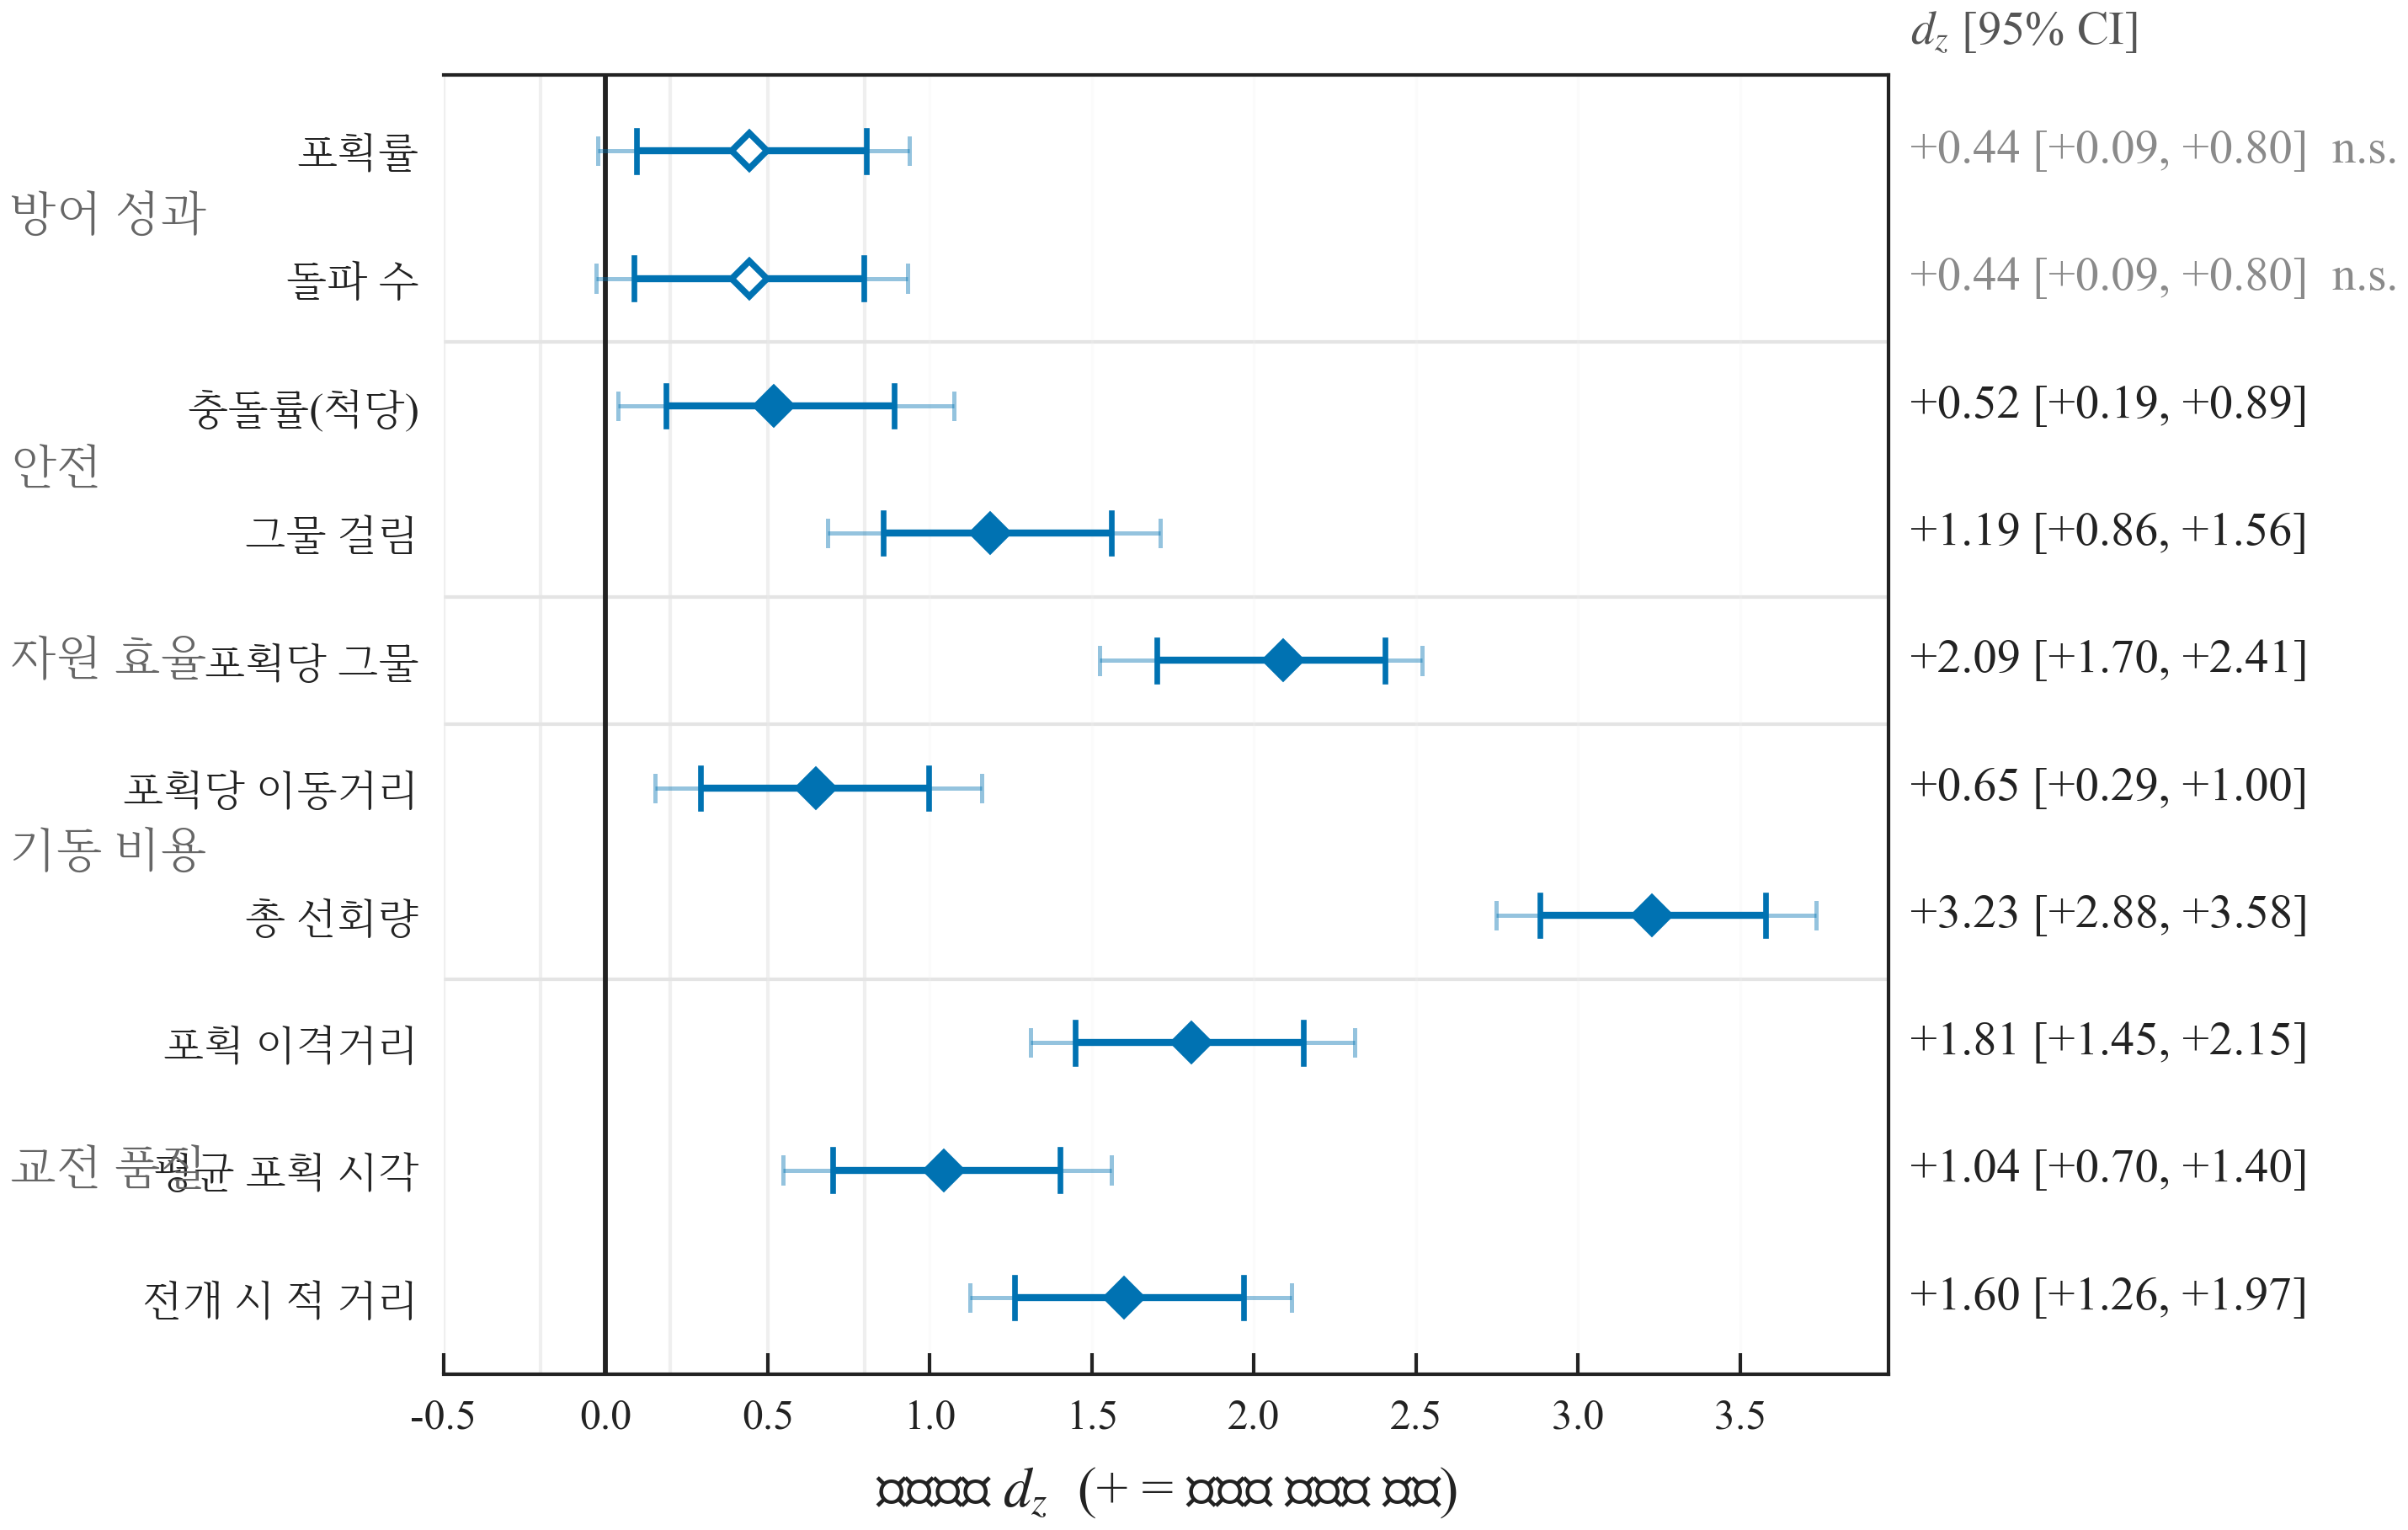
\includegraphics[width=\columnwidth]{fig23.png}
\caption{전 지표 효과크기 $\dz$(옅은 선 보정 구간)}
\label{fig:forest}
\end{figure}

개선은 포획률이 아니라 기동 비용과 자원 효율에 몰려 있다. 총 선회량은 $1625$ 에서 $868$ 로
47\,\% 줄어 $\dz = -3.23$, 포획당 그물은 45\,\% 줄어 $-2.09$, 그물 걸림은 73\,\% 줄어
$-1.19$, 포획 이격거리는 $223\unit{m}$ 늘어 $+1.81$ 이다. 반면 포획률은 $\dz = 0.44$ 로
10개 지표 중 최하위권이며 총 선회량의 7분의 1 수준이다.

다중비교 보정에서는 10개 중 8개가 그대로 유의하고, 포획률과 돌파 수만
유의성을 잃는다.

%============================================================ 7. 고찰 및 결론 (압축판)
\section{고찰 및 결론}
\label{sec:discussion}

\subsection{결과의 해석}

두 계층의 기여가 가산적이라는 것(\ref{sec:res_g3}절)은 운용상의 자유를 뜻한다. 지휘관 모델
교체와 기동 정책 재학습을 서로 기다리지 않고 독립적으로 진행할 수 있다.

지휘관의 성능을 설명하는 것은 커버리지가 아니라 재계획 간 계획 안정성이라는
관찰(\ref{sec:res_mechanism}절)은 본 문제에 국한되지 않는다. 주기적으로 재계획하는 계층
구조에서 상위 결정의 변경은 하위 계층에 전환 비용(회수되지 않는 이동과 그물)을
발생시킨다. 상위 계층이 매 재계획마다 순간 최적을 추구하면 이 비용이 누적되어, 한 번의 재계획에서 나은
배정이 에피소드 전체로는 불리해진다. 언어모델은 매 호출이 독립적이라 이 일관성이 구조적으로 보장되지
않으므로, 직전 배정을 상태에 포함시키고 담당 무리를 방위로 식별하게 한 것이 그 대응이다.
따라서 언어모델을 계획 계층에 둘 때는 계획 품질을 국소 최적성이 아니라 시간에 걸친
일관성으로 평가해야 하며, 프롬프트와 상태 표현이 그 일관성을 지원해야 한다.

가장 큰 개선이 총 선회량(\ref{sec:res_effectsize}절)에서 나타난 것은 점수맵 표현의 성질에서
온다. 경유점이 격자에 고정되므로 연속 회귀의 미세 진동이 배제되어 궤적이 부드러워지고, 선회
감소는 실제 선박에서 연료·시간·기동 여유로 환산된다. 포획당 그물 소모의 감소 역시 유효 마스크가 방위 조건과 사거리 제약을 행동 분포에 직접
부과해 무의미한 위치의 그물벽을 애초에 배제한 결과다. 다만 이 이득은 점수맵의 다봉 표현력에서 오는 것이 아니다. 유효 마스크가 남기는 셀
안에서 점수맵은 거의 단봉이며, 이득은 분포의 모양이 아니라 마스크와 격자 양자화에서 온다.

\subsection{한계와 향후 과제}
\label{sec:limitations}

검증은 시뮬레이션에 한정되며 그물 거동·얽힘 판정·관측이 단순화되어
있다(Table~\ref{tab:simfidelity}). 특히 관측 불확실성은 배정이 딛고 선 무리 구성을 흔들므로,
점수맵 정책보다 지휘관 계층에 더 크게 작용할 것이다.

가장 좋은 지휘관이 상용 폐쇄형 모델이라는 데서 오는 제약 --- 수치의 장기 재현, 능력 임계의
시점 의존성, 판단 근거 원문의 미저장 --- 은 재현성 선언에 함께 적었다.

규모는 적 10척 대 방어정 3척으로 고정이어서 방어정이 늘어 배정 조합이 급증할 때 능력 임계가
어디로 옮겨 가는지는 측정하지 않았고, 적이 규칙 기반이라 그물벽 배치를 학습해 회피하는 적응적
적은 범위 밖이다. 학습 알고리즘 비교도 같은 픽셀 행동공간 위의 MAPPO 한
종에 그치며(\ref{sec:res_algo}절), 연속 행동공간 기준선과 구성요소별 절제는 과제로 남는다.

\subsection{결론}
\label{sec:conclusion}

적보다 느린 방어정으로 자폭 군집을 막는 2계층 체계를 제안하고, 시드 대응 $2\times2$ 설계의
720 에피소드로 두 계층의 기여를 분리 측정하였다. 제안 체계는 같은 방어 수준에서 자원과 기동
비용을 크게 줄였으며, 두 계층의 기여는 가산적이었고, 언어모델 지휘관의 이득은 능력 임계 위에서만
나타났다. 실해역 이식과 관측 불확실성 하에서의 계획 안정성은 향후 과제로 남는다.

%============================================================ 자료 공개 (국방발표 판)
%  저널판(sections_real/10_declarations.tex)의 Elsevier 전용 블록 세 가지 --- CRediT 기여
%  명세, 이해관계 선언, 생성형 AI 선언 --- 은 투고 제작 시스템이 요구하는 형식 요소이므로
%  발표판에서는 싣지 않는다. 재현에 필요한 자료 공개만 남긴다.
\section*{사사}

\textcolor{red}{\textbf{[발표 전 확인 필요]}} 본 연구는 \textcolor{red}{[지원 기관·과제명·과제번호]}의
지원을 받아 수행되었다.

\section*{자료 공개}
\addcontentsline{toc}{section}{자료 공개}

본 연구의 결과를 재현하는 데 필요한 자료는 720 에피소드의 에피소드별
지표(\texttt{episodes.csv})와 계획 호출 계측값(\texttt{llm\_metrics.csv}), 기동 계층의 정책
체크포인트(\texttt{u-net\_map.pt}; 학습 설정이 체크포인트 안에 함께 저장되어 별도 설정 파일
없이 복원된다), 그리고 환경·관측 래스터화·평가 하네스를 포함한 시뮬레이터 전체다. 본문의 모든
표와 그림은 앞의 두 파일에서 기계적으로 생성되며 손으로 옮겨 적은 수치는 없다.
\textcolor{red}{[공개 URL 기입 필요]}

\vspace{3pt}
\noindent
언어모델이 생성한 판단 근거(\texttt{rationale})의 원문은
저장하지 않았고 길이만 계측하였으므로, 근거 문장 자체에 대한 사후 분석은 재현할 수
없다(\ref{sec:limitations}절). 또한 상용 API로 제공되는 폐쇄형 지휘관 모델은 버전 갱신이나
서비스 종료로 그 조건의 수치가 시점에 따라 달라질 수 있다. 언어모델을 쓰지 않는
조건(\texttt{heur\_heur}, \texttt{heur\_unet})은 이 위험 없이 재현 가능하다.

%============================================================ 참고문헌 (국방발표 판)
%  저널판(sections_real/refs.tex)에서 본문 인용이 없는 두 항목(silver2016alphago,
%  sutton2018rl)만 덜어낸 사본이다. 수동 thebibliography 라 인용되지 않은 항목도
%  목록에 찍히므로, 발표판에서는 독자가 따라갈 수 없는 항목을 두지 않는다.
%  ★ 저널판 참고문헌을 고치면 이 파일도 함께 맞출 것.
%============================================================ 참고문헌
%  natbib + 수동 thebibliography.
%  bibitem 의 대괄호에 "저자(연도)", 중괄호에 인용 키를 적는다. 그러면 본문의
%  citep 가 (저자, 연도) 로 조판된다.
%  (주석에 중괄호 예시를 쓰지 않는다 — 정합성 검사 스크립트가 실제 항목으로 오인한다.)
%
%  ★ 정렬 규칙: 이 목록의 **물리적 순서가 곧 번호**다(수동 thebibliography).
%    번호 스타일이면 최초 인용 순, 저자-연도 스타일이면 알파벳 순이어야 한다.
%    손으로 끼워 넣지 말고 python tools/sort_refs.py 로 재배열할 것.
%    (한때 번호 스타일인데 알파벳순으로 실려 30개 번호가 전부 어긋나 있었다.)
%
%  ★ 원칙: 실재를 확신하는 문헌만 싣는다. 확신 없는 인용은 넣지 않는다.
%    (초안의 사실성 원칙 A.3 을 그대로 따른다.)
\begin{thebibliography}{99}
\footnotesize
\setlength{\itemsep}{2pt}

\bibitem[Ahuja et al.(2007)]{ahuja2007wta}
Ahuja, R.K., Kumar, A., Jha, K.C. and Orlin, J.B., 2007.
Exact and Heuristic Algorithms for the Weapon-Target Assignment Problem.
\textit{Operations Research}, 55(6), pp.1136--1146.

\bibitem[Wang et al.(2021)]{wang2021cuas}
Wang, J., Liu, Y. and Song, H., 2021.
Counter-Unmanned Aircraft System(s) (C-UAS): State of the Art, Challenges, and
Future Trends.
\textit{IEEE Aerospace and Electronic Systems Magazine}, 36(3), pp.4--29.

\bibitem[Sutea(2026)]{sutea2026fiber}
Sutea, V., 2026.
\textit{Fiber-optic drones have emerged as critical kit for both Russia and
Ukraine}. Atlantic Council UkraineAlert, 24 February 2026.

\bibitem[Rumbaugh(2024)]{rumbaugh2024cost}
Rumbaugh, W., 2024.
\textit{Cost and Value in Air and Missile Defense Intercepts}.
Washington, DC: Center for Strategic and International Studies (CSIS) Commentary,
13 February 2024.

\bibitem[Kuhn(1955)]{kuhn1955hungarian}
Kuhn, H.W., 1955.
The Hungarian Method for the Assignment Problem.
\textit{Naval Research Logistics Quarterly}, 2(1--2), pp.83--97.

\bibitem[Liu et al.(2016)]{liu2016usv}
Liu, Z., Zhang, Y., Yu, X. and Yuan, C., 2016.
Unmanned surface vehicles: An overview of developments and challenges.
\textit{Annual Reviews in Control}, 41, pp.71--93.

\bibitem[Zhang et al.(2025)]{zhang2025encircle}
Zhang, C., Zeng, R., Lin, B., Zhang, Y., Xie, W. and Zhang, W., 2025.
Multi-USV cooperative target encirclement through learning-based distributed
transferable policy and experimental validation.
\textit{Ocean Engineering}, 318, 120124.

\bibitem[Lowe et al.(2017)]{lowe2017maddpg}
Lowe, R., Wu, Y., Tamar, A., Harb, J., Abbeel, P. and Mordatch, I., 2017.
Multi-Agent Actor-Critic for Mixed Cooperative-Competitive Environments.
\textit{Advances in Neural Information Processing Systems 30 (NeurIPS)}.

\bibitem[Rashid et al.(2018)]{rashid2018qmix}
Rashid, T., Samvelyan, M., Schroeder de Witt, C., Farquhar, G., Foerster, J. and
Whiteson, S., 2018.
QMIX: Monotonic Value Function Factorisation for Deep Multi-Agent Reinforcement
Learning.
\textit{International Conference on Machine Learning (ICML)}, pp.4295--4304.

\bibitem[Foerster et al.(2018)]{foerster2018coma}
Foerster, J., Farquhar, G., Afouras, T., Nardelli, N. and Whiteson, S., 2018.
Counterfactual Multi-Agent Policy Gradients.
\textit{AAAI Conference on Artificial Intelligence}, pp.2974--2982.

\bibitem[Yu et al.(2022)]{yu2022mappo}
Yu, C., Velu, A., Vinitsky, E., Gao, J., Wang, Y., Bayen, A. and Wu, Y., 2022.
The Surprising Effectiveness of PPO in Cooperative Multi-Agent Games.
\textit{Advances in Neural Information Processing Systems 35 (NeurIPS)}.

\bibitem[Schulman et al.(2017)]{schulman2017ppo}
Schulman, J., Wolski, F., Dhariwal, P., Radford, A. and Klimov, O., 2017.
Proximal Policy Optimization Algorithms.
\textit{arXiv preprint arXiv:1707.06347}.

\bibitem[Haarnoja et al.(2018)]{haarnoja2018sac}
Haarnoja, T., Zhou, A., Abbeel, P. and Levine, S., 2018.
Soft Actor-Critic: Off-Policy Maximum Entropy Deep Reinforcement Learning with a
Stochastic Actor.
\textit{International Conference on Machine Learning (ICML)}, pp.1861--1870.

\bibitem[Shao et al.(2024)]{shao2024deepseekmath}
Shao, Z., Wang, P., Zhu, Q., Xu, R., Song, J., Bi, X., Zhang, H., Zhang, M.,
Li, Y.K., Wu, Y. and Guo, D., 2024.
DeepSeekMath: Pushing the Limits of Mathematical Reasoning in Open Language Models.
\textit{arXiv preprint arXiv:2402.03300}.

\bibitem[Long et al.(2015)]{long2015fcn}
Long, J., Shelhamer, E. and Darrell, T., 2015.
Fully Convolutional Networks for Semantic Segmentation.
\textit{IEEE Conference on Computer Vision and Pattern Recognition (CVPR)},
pp.3431--3440.

\bibitem[Ronneberger et al.(2015)]{ronneberger2015unet}
Ronneberger, O., Fischer, P. and Brox, T., 2015.
U-Net: Convolutional Networks for Biomedical Image Segmentation.
\textit{Medical Image Computing and Computer-Assisted Intervention (MICCAI)},
pp.234--241.

\bibitem[Liu et al.(2018)]{liu2018coordconv}
Liu, R., Lehman, J., Molino, P., Petroski Such, F., Frank, E., Sergeev, A. and
Yosinski, J., 2018.
An Intriguing Failing of Convolutional Neural Networks and the CoordConv Solution.
\textit{Advances in Neural Information Processing Systems 31 (NeurIPS)}.

\bibitem[Perez et al.(2018)]{perez2018film}
Perez, E., Strub, F., de Vries, H., Dumoulin, V. and Courville, A., 2018.
FiLM: Visual Reasoning with a General Conditioning Layer.
\textit{AAAI Conference on Artificial Intelligence}, pp.3942--3951.

\bibitem[Vinyals et al.(2015)]{vinyals2015pointer}
Vinyals, O., Fortunato, M. and Jaitly, N., 2015.
Pointer Networks.
\textit{Advances in Neural Information Processing Systems 28 (NeurIPS)}.

\bibitem[Vaswani et al.(2017)]{vaswani2017attention}
Vaswani, A., Shazeer, N., Parmar, N., Uszkoreit, J., Jones, L., Gomez, A.N.,
Kaiser, {\L}. and Polosukhin, I., 2017.
Attention Is All You Need.
\textit{Advances in Neural Information Processing Systems 30 (NeurIPS)}.

\bibitem[Huang et al.(2022)]{huang2022zeroshot}
Huang, W., Abbeel, P., Pathak, D. and Mordatch, I., 2022.
Language Models as Zero-Shot Planners: Extracting Actionable Knowledge for
Embodied Agents.
\textit{International Conference on Machine Learning (ICML)}, pp.9118--9147.

\bibitem[Ahn et al.(2022)]{ahn2022saycan}
Ahn, M., Brohan, A., Brown, N., et al., 2022.
Do As I Can, Not As I Say: Grounding Language in Robotic Affordances.
\textit{Conference on Robot Learning (CoRL)}.

\bibitem[OpenAI(2026)]{openai2026function}
OpenAI, 2026. \textit{Function calling}. [Online]
Available at: \texttt{https://developers.openai.com/api/docs/guides/function-calling}
[Accessed 9 August 2026].

\bibitem[Wu and He(2018)]{wu2018groupnorm}
Wu, Y. and He, K., 2018.
Group Normalization.
\textit{European Conference on Computer Vision (ECCV)}.

\bibitem[Ng et al.(1999)]{ng1999shaping}
Ng, A.Y., Harada, D. and Russell, S., 1999.
Policy Invariance Under Reward Transformations: Theory and Application to
Reward Shaping.
\textit{International Conference on Machine Learning (ICML)}, pp.278--287.

\bibitem[Loshchilov and Hutter(2017)]{loshchilov2017sgdr}
Loshchilov, I. and Hutter, F., 2017.
SGDR: Stochastic Gradient Descent with Warm Restarts.
\textit{International Conference on Learning Representations (ICLR)}.

\bibitem[Fossen(2011)]{fossen2011marine}
Fossen, T.I., 2011.
\textit{Handbook of Marine Craft Hydrodynamics and Motion Control}.
Chichester: John Wiley \& Sons.

\bibitem[Efron and Tibshirani(1993)]{efron1993bootstrap}
Efron, B. and Tibshirani, R.J., 1993.
\textit{An Introduction to the Bootstrap}. New York: Chapman \& Hall.

\bibitem[DiCiccio and Efron(1996)]{diciccio1996bca}
DiCiccio, T.J. and Efron, B., 1996.
Bootstrap Confidence Intervals.
\textit{Statistical Science}, 11(3), pp.189--228.

\end{thebibliography}

% 영문 초록은 국내 논문 관례대로 맨 뒤.
% 2026-09-16 제외 --- 국문 원고 끝의 영문 초록은 싣지 않는다(영문판은 00b 파일에 보존).
% %============================================================ 영문 표제·초록
%  EAAI 는 영문 저널이다. 이 한글 원고는 투고본의 기준 원고이므로, 번역 단계에서
%  용어와 수치가 흔들리지 않도록 영문 제목·초록·주제어를 여기에 고정해 둔다.
%  ★ 수치는 국문 초록과 한 글자도 다르면 안 된다 — tools/check_paper_meta.py 가 대조한다.
%  ★ 이 파일은 투고 원고에 들어가지 않는다 — elsarticle 에는 본문 뒤 제2 초록에
%    대응하는 요소가 없다. 독립 문서 영문초록_translation_reference.tex 가 읽는다.

\section*{English Abstract}
\addcontentsline{toc}{section}{English Abstract}

% 14.4pt 볼드 한 줄로는 판면을 넘는다. 줄바꿈을 손으로 준다.
\noindent\textbf{\large LLM-Based Command Architecture and U-Net Score-Map\\
Multi-Agent Cooperative Reinforcement Learning\\
for Defense Against Suicide USV Swarms}

\vspace{4pt}
\noindent
Low-cost suicide unmanned surface vehicle (USV) swarms evade conventional counters:
electronic warfare cannot reach wire-guided targets, and interceptors cost more than their
targets and saturate. We propose a two-layer defense in which a few boats slower than the
attackers pre-block the mothership approach corridor with net walls. In the strategy layer a
large language model (LLM) commander assigns each boat to an enemy cluster; in the maneuver
layer a U-Net emits a score map over a rasterized battlefield grid and each boat points at
pixels to place its net wall. Both layers update on the same period but differ sharply in
response latency, so only the slow strategy layer is decoupled asynchronously. Pixel pointing
confines the action space to the grid, imposes safety constraints by masking, and is
invariant to swarm size; training extends critic-free group relative policy optimization to
the multi-agent case. With no combinatorial post-optimization, we collected
720 seed-paired episodes (8 conditions $\times$ 3 formations $\times$ 30 seeds) and separated
the two layers' contributions in a $2\times2$ decomposition. The maneuver layer alone raised
capture rate from $0.844$ to $0.886$; the full system cut nets per capture by 44.5\,\% and total
turning by 46.6\,\% at the same defense level, and the two contributions were \emph{additive}
rather than synergistic. The commander paid off only above a capability threshold: a cloud
model gained $+0.060$, whereas local Qwen2.5 7B was significantly worse than the code heuristic
at $-0.192$. Commander performance was explained by plan stability across replans, not by
assignment coverage: in periodically replanning architectures, temporal consistency matters
more than local optimality.

\vspace{4pt}
\noindent\textbf{Keywords}\;:\;
unmanned surface vehicle; swarm defense; multi-agent reinforcement learning; task assignment;
large language model; semantic segmentation; group relative policy optimization

\vspace{6pt}
\noindent\textbf{Highlights}
\begin{itemize}[leftmargin=1.1em, itemsep=1pt, topsep=2pt, parsep=0pt]
\item Two judgment layers share one 25 s period; only the slow one is decoupled
\item Pointing at score-map pixels keeps the action space invariant to swarm size
\item Critic-free, heuristic-anchored group relative optimization for multi-boat coordination
\item Across 720 paired episodes the two layers are additive in 9 of 10 metrics
\item Commander skill is explained by plan stability, not assignment coverage
\end{itemize}


\end{document}
